\documentclass[a4paper, svgnames]{article}

\usepackage[a4paper, margin=1in]{geometry}
\usepackage[english]{babel}
\usepackage[utf8x]{inputenc}
\usepackage{amsmath}
\usepackage{graphicx}
\usepackage[colorinlistoftodos]{todonotes}
\usepackage{sectsty}
\usepackage{float}
\usepackage{natbib}
\usepackage{url}
\usepackage[colorlinks]{hyperref}
\usepackage{xcolor}
\usepackage{amsmath}
\usepackage{longtable}
\setlength\LTcapwidth{\textwidth}
\usepackage{pdflscape}
\usepackage{booktabs}
\usepackage{afterpage}
\usepackage[bottom]{footmisc}
\usepackage{tikz}
\usepackage{multirow}
\usepackage{enumitem}
\usepackage{bibspacing}
\setlength{\bibitemsep}{0\baselineskip plus .05\baselineskip minus .05\baselineskip}
\usepackage{rotating, float, placeins}
\usepackage{threeparttable}
\widowpenalty10000
\clubpenalty10000

% Node styles
\tikzstyle{basic box}=[fill=none, draw=black, shape=rectangle]

% Edge styles
\tikzstyle{basic arrow}=[fill=black, ->]

\hypersetup{
    colorlinks,
    citecolor=Blue,
    linkcolor=Blue}

\linespread{1.25}
\sectionfont{\large}
\setlength{\parskip}{1mm}

\newcommand{\citeposs}[1]{\citeauthor{#1}'s \citeyearpar{#1}}
\newcommand{\citepos}[1]{\citeauthor{#1}' \citeyearpar{#1}}

\title{\vspace{-40pt}\textbf{The consequences of affective polarization\\ \Large Is accountability still working?}}
\author{Rodrigo Fernández Caba}
\date{\vspace{-5pt} July, 2022}

\begin{document}
\maketitle

\begin{abstract}
	Affective polarization has become the political phenomenon of the moment. Although specially American scholars have studied thoroughly its causes, less effort has been devoted to explain its consequences. In order to do so, I propose a causal mechanism through which affective polarization impacts political attitudes. By a process of motivated reasoning, more polarized people are expected to a) assess incumbent's performances worse, b) form political preferences (i.e. public policy choice) in a perhaps pernicious way for them, and c) be less supportive in general for incumbent's measures (specially during times of crisis). In this paper, I propose to test empirically the first of these effects, namely, the impact of affective polarization on economic voting. My hypothesis is that those who are more polarized will be less rational or, in other words, they will be less able to reward or punish the incumbent according to economic events. Hence, this paper tries to make a contribution to our knowledge of affective polarization and speaks to the general problem of accountability in our contemporary polarized societies.
\end{abstract}


\section{Introduction}

Some scholars have recently pointed out that American people are far more polarized than 40 years ago \citep{Lelkes2018}. Since the seminal piece of work by \cite{Iyengar2012} we know that political polarization is not only related to ideology but also to affects. Inter-party animosity has been increasing at least since the 1980s in American politics. Nonetheless, some others have shown that United States is by no means the most polarized nation around the world. From a comparative perspective, (\citeauthor{Gidron2018} \citeyear{Gidron2018} and \citeyear{Gidron2019}, and \cite{WESTWOOD2018}) (see Figure \ref{fig:af-pol-comp}) have pointed out that whereas Americans display just average levels of affective polarization, in Europe, we find much higher levels, for instance, in countries like Spain, Greece or even France. The ugly discourse surrounding recent elections in the US, the Brexit campaign, or the regional elections in Community of Madrid (Spain) on may 2019, held in a frame with only two apparent options `Communism or Freedom', are just some examples of the increasingly divisive political discourse of our times. What we call affective polarization is, loosely speaking, the phenomenon that voters like their political co-partisans and, usually at the same time, they dislike their political opponents, that is, they see themselves belonging to an in-group and therefore, they dislike (or sometimes even hate) the out-group members.

\begin{figure}
	\centering
	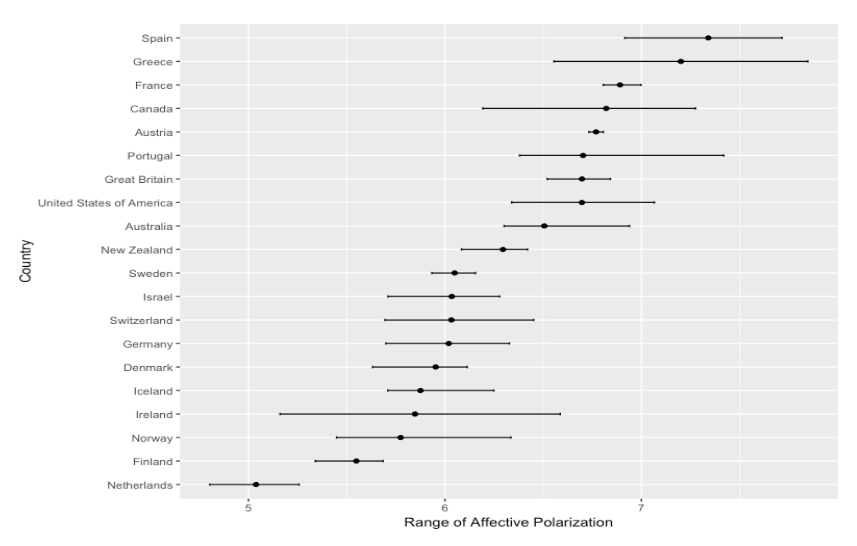
\includegraphics[scale=.7]{figure1.png}
	\caption{\label{fig:af-pol-comp} Levels of affective polarization across countries. Source: \cite{Gidron2018}}
\end{figure}

Affective polarization has been well-documented since 2012 --specially regarding its causes--, at least in the US \citep{Hetherington2015,Rogowski2016a, Webster2017,Lelkes2018,Iyengar2019, Klein2020}. However, scholars in Europe --and also in Spain-- have only started to focus on this issue recently, although as \cite{Miller2019} points out, the prominence of the concept makes it the ``political phenomenon of the moment". Moreover, little effort has been made investigating the consequences of the phenomenon. Perhaps, the reason behind the lack of studies focused on the consequences of affective polarization is related to poor data (that is the case of Spain), or that's simply because it is a very complex phenomenon that depending on the country can be very correlated with simple ideological polarization and other similar phenomena, making it difficult to disentangle its effects. Others have even suggested that affective polarization does not have such political consequences \citep*{broockmanDoesAffectivePolarization2020}, and hence, there is no reason to explore them. However, some facts point towards the opposite direction and we have already measured the increasing levels of polarization. For example, we already know that 2008 financial crisis had a great impact on the european party systems. In some places like Spain, after more than two decades of stable bipartidism, a multiparty system emerged. This increase in the number of parties confronting in parliament happened after a sharp increase of affective polarization which, in the case of Spain, has ended up leading spanish people to polarize even more in two big blocks of parties \citep{Orriols2020}.

The majority of studies addressing this question points out that high levels of affective polarization could be dangerous for democracy. Scholars usually argue that it makes democracy work worse although they do not usually test in which way. This lack of theoretical contributions leading towards empirical ways of looking for the consequences of affective polarization is what mainly inspire this work. Some exceptions are worth noting, though: \cite{Wagner2021} finds that affective polarization has an impact on democratic values. Specifically, he finds a negative effect on satisfaction with democracy. Similarly, \cite{Ward2019} find that affective polarization affects perceptions of political choice as well as turnout and participation. But taking these exceptions aside, most of the comments in the literature so far are closer to be intuitions than proper empirical findings. For instance, there is a common intuition in the literature that polarized citizens are less able to collaborate and to work together to solve collective action problems \citep{Garrett2014}. Citizens' trust in political institutions and legitimacy of governments might also be negatively affected \citep{Orriols2021}. In the same vein, affective polarization can also foster political radicalism \citep{Levendusky2013, Rogowski2016a, Webster2017} since the dynamics of polarized politics makes the radicals more prone to speak and, at the same time, it makes polarized --but less radical-- people, more prone to follow the former. There is also a concern regarding satisfaction with democracy, electoral participation, and a long list of attitudes towards western liberal electoral democracy. However, most of those are just intuitions or ideas derived from the analysis of the causes of affective polarization, and since almost none of those pernicious effects of affective polarization have been \textbf{empirically} tested, this study tries to first ask if any of those suggested political consequences are playing a role in electoral terms and if so, how does affective polarization really operates. Specifically, in this paper I focus in which is arguably the most concerning of all possible consequences in electoral terms, that is, to what extent accountability mechanisms are affected by this phenomenon, hence I explore its relationship with economic voting and attribution of responsibility.

The general argument is that affective polarization makes people assess political phenomena --and also non-political phenomena-- using their own `political glasses'. Hence, they are less permeable to political information and political cues, or in other words, they are less prone to process political information from a critical standpoint. We already know that partisanship impacts the way in which people hold incumbents accountable \citet*{tilleyGovernmentBlameExperimental2011a}. The fact that people feel very attached to a certain party, has been proved to bring this kind of polarization, however, when polarization is based not only on the identification with a party but also on affects and especially on the animosity towards the out-group (as I will explain below), these already known effects might, I argue, be even more pronounced and, consequently, worse for democracy. 

As I will develop in subsequent sections, the basic idea is that our own political (partisan) biases, are exacerbated when we identify an (social) in-group to which we belong, and an (social) out-group that we see as totally opposed to us, that is, political militancy turns into identity. This situation reduces our critical assessment of political --and non-political-- phenomena, or more precisely, it makes us use this assessment (correct or not and based on relatively objective information) to a lesser extent when it comes to hold incumbents accountable. In short, affective polarization would make people use their assessment of the economy in such a way that they avoid punish their in-group and/or they punish their out-group harder than economic situation might predict.

Hence, the goal of this study is twofold: first, I propose a theoretical mechanism that explains why affective polarization has negative effects on the democratic process, specifically on the degree to which people is able to hold incumbents accountable according to economic performance and I test it empirically. And second, I explore the dynamics of positive and negative partisanship, the constituents of affective polarization in Spain during crucial political times. According to the argument, we should see polarized people unable to reward or punish incumbents according to economic performance, that is, we should observe that accountability does not work properly. The remaining of this study proceed as follows: first I present my argument discussing the relevant literature on affective polarization and economic voting. Second, I present my data and experimental design. In a subsequent section I discuss the main results. Finally, I conclude.

\section{Understanding affective polarization}
\label{affective polarization}

Affective polarization is a fairly new field of research. The concept relates to the fact that citizens feel sympathy towards a partisan in-group and antagonism towards a partisan out-group \citep{Wagner2021}. Regardless of its novelty, it has been largely studied in the US. After the work of \cite{Iyengar2012} came out, a lot of different aspects of this phenomenon have been empirically tested in many different countries. However, the vast majority of the literature has focused on the causes, and only a few instances have said something abut its consequences. Also, given the salience of the topic in American politics, scholars have measured affective polarization \footnote{To see a more in depth discussion on the concern about how to measure affective polarization see \cite{Druckman2019}} mostly in the arguably most straightforward case, the american two-party system \citep{Wagner2021}. However, some authors have recently tried to fill this gap and they have proposed new ways of measuring it in multi-party systems \citep{Reiljan2020}. Moreover, affective polarization is usually addressed at the aggregate level, that is, as the average affective polarization of the political system. Nonetheless, it can also be studied from an individual perspective, since in the end, each individual has a level of affect (or disaffect) for these in-group and out-group members. \citep{Wagner2021}.

So far, we know that affective polarization is more complex that one might think at first glance. It is neither ideological polarization (although correlation is high in certain contexts), nor party identification (although this is an essential part of it). It is rather something related to social identity. Therefore, it is rooted in political psychology and more precisely in social identity theory \citep{Tajfel1979}. From this standpoint, affective polarization relates to the belonging sentiment to certain social groups. Although it can be the case that belonging to a social group is a matter of ideology, affective polarization is not exactly the same as ideological polarization since specially in a multiparty context, people who belong to the same part of the ideological spectrum can have different in- and out-groups for different reasons. In fact, as some scholarship has shown, in some settings affective polarization can increase while ideological divisions shrink \citep{Levendusky2016, Iyengar2019}. Nonetheless, some other scholarship has shown that ideological polarization somehow impacts affective polarization \citep{Rogowski2016a, Webster2017}.

Moreover, affective polarization is not only party identification (i.e. positive in-group affect towards a party and its supporters) because it also relates to the positive or negative out-group affect towards other parties and their supporters. That is, as some have already pointed out \citep{Medeiros2013, Abramowitz2016}, there is `negative partisanship' as well as positive partisanship. Moreover, specially in multiparty systems (in which I am interested here) the in-group and the out-group are not necessarily conformed by one single party each. On the contrary, there can be several combinations regarding the number and the distribution of parties in those groups and, even more importantly, these combinations may be related to country's cleavages in specific contexts and moments like, for instance, Spain and the Catalan secessionist movement during the last 5 years.

\section{Economic voting revisited}

Contrary to what happens with affective polarization, economic voting is not a new issue. According to \cite{LewisBeck2007}, we can find studies dating as far back as 1878. But the pioneer papers on the topic are very well known since the 1930s \citep{Tibbitts2015, Gosnell1940, Wilkinson1950}. However, the first scientific proposition of the relationship between the economy and electoral results was placed in a chapter of the seminal \textit{The American Voter} by Campbell et al. (\citeyear[Chapter 14]{campbellAmericanVoter1960}), where they even suggest that economic prosperity is associated to the incumbent presidential party. Since then, a huge literature has been produced on economic voting. Moreover, the classical theory has received considerable empirical support \citep{Kinder1979, Lewis-Beck1988, Lewis-Beck2000, LewisBeck2007, Lewis-Beck2011}. The basic claim of this theory is based on rational choice theory and says that voters, trying to maximize their utility, would vote accounting for the government economic performance. This is usually understood as one of the main accountability mechanisms in western liberal democracies. When economy goes bad, voters punish incumbents, whereas when they do well, voters reward them.

A similar way of putting the core argument of this theory is looking at one of the main `stylized facts' about economic voting, which is the following: retrospective voting is usually more important than prospective voting \citep{Lewis-Beck2000}. This is sometimes called the `responsibility hypothesis': voters hold the government responsible (i.e. accountable) for economic events. Hence, according to this theory, we should observe that voters properly assess the performance of the incumbent and vote accordingly.

However, some scholarship has already pointed out that economic voting is influenced by the context \citep{Dorussen2002, Anderson2007, Singer2015}. \cite{Dorussen2002} argue that the most explosive growth of the economic-voting literature was, interestingly, related to the emergence of controversies about the nature of the economic-voting calculus. Although previous literature had proved that economic performance had such an important salience among the electorate to influence election outcomes, it was not clear which economic policies matter most to voters. Also, it was far from clear if this salience varies across groups of voters, electoral contexts and political systems \citep{Dorussen2002}.

According to this literature, we shouldn't look at the relation between vote and economy isolated, but accounting for contextual factors. As \citet[p. 1]{Singer2015} point out, ``there is still a debate about whether voters focus on past or future performance and whether they view the economy in primarily sociotropic or egotropic terms". They find that prospective voting predominates early in the election cycle and retrospective voting gains traction as people observe incumbent's performance. Moreover, they also find that sociotropic views predominates over the egotropic ones except for the least developed countries. In the same vein, in a provocative paper, \cite[p. 1]{Anderson2007} argues that economic voting does not work as `envisioned by advocates of democratic accountability'. He  calls for a reconsideration of the normative underpinnings of economic voting paradigm in light of recent evidence. His argument is that although the findings supporting empirically the theory enumerated above exist, they are contingent for both institutional and psychological reasons. Precisely building on that argument, I try to disentangle both potential reasons in this study and I focus specifically on the latter. That is, as suggested above, although economic voting works in general, it can fail under certain circumstances, I argue that a context with high levels of affective polarization --through psychological biases-- is one of those.

The core empirical assumption of the economic voting theory still holds: it is more likely to find people voting retrospectively than prospectively. Only when people observe incumbent's performance they start thinking in voting in prospective terms. As I would argue in the next section more in depth, it is reasonable to expect that retrospective voting (and economic voting in general) work worse as people are more polarized. This is to say that as people become more affectively polarized they use the economy to a lesser extent in order to make an electoral decision. The idea behind this rationale follows the logic proposed by \citet*{tilleyGovernmentBlameExperimental2011a} when analyzing the role played by partisan bias when assessing public policy. Partisan biases might impact either the assessment of the economy the individual makes, how she attributes responsibility or even both. These two things, however, yield different models of electoral accountability and have different consequences.

Their general theory suggests two (non-exclusionary) possibilities. On the one hand, people could be less able to assess the state of the economy and hence, they will vote according to a biased assessment. That means that they are rational enough as to vote according to their assessment, so \textit{stricto sensu} the economic voting mechanism would work as expected; it is rather their evaluation of the economy what is wrong, that is, contrary to objective markers. They would ignore objective economic data to avoid punishing the incumbent. On the other hand, they could correctly assess the economy but --trying to minimize the subsequent cognitive dissonance-- they attribute responsibility in a partisan way. That is, they evaluate the economy according to objective economic parameters but exonerate the government if it belongs to their party. The former is known as the \textbf{selective evaluation} model whereas the latter is known as the \textbf{selective attribution} model. According to the theory I propose here, the latter is thought to be playing a prominent role. It is not that polarized people assess the economy wrongly but rather that even when they evaluate the economy correctly, the more polarized they are, the less important the economy is in their final decision.

This --I argue-- should be especially true and clear for the case of incumbent supporters. The fact that elections are used as a mechanism of accountability makes us expect people to punish or reward incumbents according to the state of the economy (basic economic voting mechanism). However, the more affectively polarized people is, the harder it is for them to punish the incumbent when it belongs to their in-group. Simply because affective polarization is linked to social identity, people would exonerate to a larger extent the incumbent if they think the economy goes bad, usually attributing responsibility in a wrong or, at least, biased way. I expect to see voters to use some other strategies and shortcuts in order to maximize their utility, so polarized individuals should avoid to a larger extent the use of information to make their final decision and cast their votes.

\section{Argument}

Once I have presented the most relevant literature to understand affective polarization and economic voting, the linking nexus must be analyzed. I argue that affective polarization has a direct effect on political attitudes, more specifically on the extent to which individuals use new performance information to ultimately cast their votes, because it activates a process of motivated reasoning (see Figure \ref{fig:model}). This effect is similar in essence to the already known partisan bias present in  \citet*{tilleyGovernmentBlameExperimental2011a}'s models of accountability. However, I think that it is not only partisan identification but also polarization --and specifically polarization based on affects-- what may affect economic voting. These two things are not the same as suggested above basically because polarization may be caused due to good feelings towards the in-group (positive partisanship) but also negative feelings towards the out-group (negative partisanship). Moreover, in multiparty settings like Spain, these groups do not coincide necessarily with only one party each, what makes the effect if it exists, even more important than suggested in the models by \citet*{tilleyGovernmentBlameExperimental2011a}.

The basic idea is that even when citizens might correctly assess the state of the economy, they will avoid to punish their in-group --and consequently the incumbent-- electorally. In other words, the state of the economy or government performance becomes less important for those supporting the incumbent the more polarized they are. They become more inelastic to economic (or performance-based more in general) information. Although the theory affects everyone voting, in order to empirically test my theoretical expectations we restrict to incumbent supporters from this point on. This is basically because I am interested in an accountability mechanism which is mainly related to those who being incumbent supporters eventually might either reward or punish it.

\begin{figure}[H]
	\centering
	\begin{tikzpicture}
		\node  (0) at (-5, 0) {Affective Polarization};
		\node  (1) at (0, 0) {Motivated Reasoning};
		\node  (2) at (5.5, 0) {Less economic voting};

		\draw [style=basic arrow] (0) to (1);
		\draw [style=basic arrow] (1) to (2);

	\end{tikzpicture}
	\caption{\label{fig:model} Effect of affective polarization on Economic Voting}
\end{figure}

\subsection{Motivated reasoning}

Motivated reasoning is usually studied in cognitive science and social psychology and refers to the fact that some people use emotionally biased reasoning to produce justifications (or make decisions) that are most desired rather than those that accurately reflect the evidence \citep{Kunda1990}. In my setting, this is reflected by the fact that `affectively' polarized people are so according to their emotions, that is, to the level of animosity against both the in-group and the out-group. They would use motivated reasoning to avoid being at odds with their in-group. They would prefer to be `loyal' to their in-group than to punish them if economic situation goes bad. Or the other way around, they would avoid rewarding their out-group when economic performance was good. In other words, those more polarized are expected to use motivated reasoning to a larger extent and hence, would be less able to process (i.e. evaluate) and integrate political (or economic) information. They will be less willing to hold their party accountable for policy performance. That is, this motivated reasoning would lead them to vote in a less rational way, or in other words, accountability based on economic voting will work worse. It is reasonable to expect partisans to undermine rather than promote responsible government.

As suggested by many scholars \citep{Taber2006, Boyer}, reasoning seems to play a crucial role in the formation of political attitudes. Citizens are not only motivated in the sense of holding \textit{accurate} beliefs, but also ``\textit{directional} motivations, or motivations to reach a certain predetermined belief" \citep[p.2]{Boyer}. Such directional motivations are, according to \cite[p. 440]{Kunda1990}, ``any wish, desire or preference that concerns the outcome of a given reasoning task". In order to better understand the underpinnings of the process by which polarized people activate a motivated reasoning process, it is interesting to discuss the different effects that positive and negative partisanship may have.

If we look at the characterization of motivated reasoning proposed by \cite{Thaler2021}, we would find that the causal chain proposed in Figure \ref{fig:model} is valid. He argues that motivated reasoning ``posits that people distort their inference process in the direction of states they find more attractive". Taking this characterization, we see that people activate the motivated reasoning process once they find a state considered as ``more attractive". Thus, since affective polarization is a byproduct of the in-group and out-group feelings, or rather, of positive and negative partisanship, this context of affective polarization is required prior to motivate the reasoning. Put it differently, only once people is polarized because they like or dislike a certain party or set of parties (and maybe their supporters), they can motivate their reasoning when assessing, for instance, economic events. The bias is produced once they know which is their in-group and out-group and only then, they direct themselves to a certain state they find more attractive. However, I argue that people is able (in general) of making a (to a large extent) accurate assessment of the economy, what directional motivated reasoning is causing according to my theory is that these people do not use this assessment to cast their votes. As I develop in the next section, people become more inelastic the more polarized they are.

\subsection{Elasticity}

I introduce now the concept of elasticity to try to shed light on the economic voting part of the argument. I use the term elasticity to refer to the extent to which people is permeable to political information. According to my argument, polarized people are, in general, less permeable to political information, specially when this information is at odds with their prior beliefs. This is to say --in bayesian terms-- that they (almost) do not update their priors. Moreover, I argue that when political polarization is not only about policy choice, but also related to affects, (lacking) permeability turns into (lacking) elasticity. These two concepts may look the same at first glance but it is not only a matter of nouns. I use elasticity instead of permeability because I characterize the relationship between economic assessment and accountability as either elastic or inelastic in the following sense: if someone is able to properly assess the state of the economy (according to objective economic markers) the fact that this individual uses this evaluation to either punish or reward the incumbent is what makes her more or less elastic. If they update their beliefs according to their evaluation and vote accordingly, they are elastic. Conversely, if they do not use their evaluation in order to cast their votes, they are inelastic to performance-based information.

\subsubsection{Elasticity and positive and negative partisanship}

Elasticity is then directly affected by the amount of affective polarization an individual displays. The more affectively polarized someone is, the less elastic he or she should be. And since affective polarization can be conceptualized as a distance between the in-group and the out-group, we can further distinguish between amount and types of affective polarization. As stated above, affective polarization is not necessarily caused only by the in-group or the out-group, but it is generally a combination of both. This can yield different results and profiles, whereas the level of affective polarization is an absolute number capturing the \textit{amount} of polarization, this amount can be separated into two ``components'' or what I call \textit{types} of affective polarization. There are people that is polarized because they like their in-group very much (i.e. positive partisanship), people that is polarized because they dislike their opponents a lot, or even hate them (i.e.  negative partisanship) or a combination of both. The latter would be the most \textit{clearly} polarized in the sense that both effects are playing a role. People with this profile like their in-group and dislike their out-group at the same time, which in turn should be the most common case. The other two profiles are less common and would represent people whose level of polarization is due to only one of the two components.

Please note that this does not mean that the level of polarization is smaller in the latter case. The amount of polarization can be as large as the sum of the two components is (the module of the diagonal vector, or the hypotenuse of the triangle; see Figure \ref*{fig:types_and_levels_of_AP}). The two types are independent of each other in the sense that they could be different and also equal to each other. There are people whose in-group feelings and out-group feelings are similarly large, and people whose animosity towards one of the groups is substantially larger and is what ultimately drives his/her polarization level. This would have qualitative consequences but, in quantitative terms, there is an infinite number of combinations of these two components. What I argue here is that the total amount of polarization can only be due to either negative partisanship or positive partisanship, and also that either of the two can be null\footnote{In this case, affective polarization is only due to one of the two groups, either the in-group or the out-group.}.

Although it is reasonable to expect that --in general terms-- partisans will be more inelastic than non-partisan voters, the interesting part of the argument is the extent to which affective polarization moderates the level of economic voting of those who identify with the incumbent. Hence, restricting ourselves to the incumbent voters, it is expected to find what I call \textit{supporters}, people with average to high levels of elasticity; what I call \textit{regular partisans} with average levels of (lack of) elasticity and \textit{fans}, with very low levels of elasticity. The first profile would be able to either punish or reward the incumbent according to economic performance. The second profile would be less so and the last one might be unable to critically use the economy as an accountability mechanism. In short, elasticity is a function of positive and negative partisanship. One of the goals of the present study is to disentangle these effects in order to better understand affective polarization when it is decomposed in its two constituent components.

\begin{figure}[H]
	\centering
	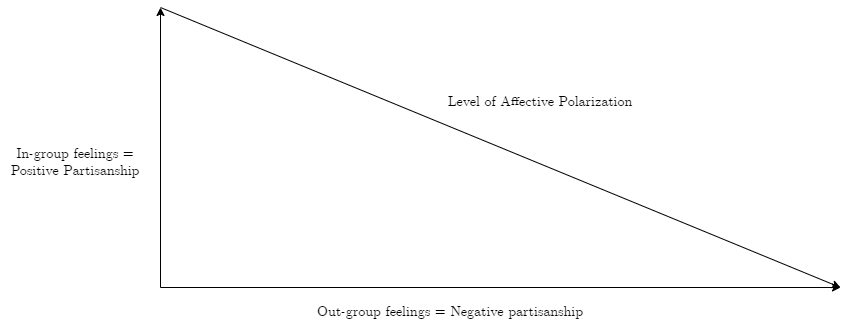
\includegraphics[scale=0.55]{Figures/AP.drawio.png}
	\caption{Types and levels of Affective Polarization}
	\label{fig:types_and_levels_of_AP}
\end{figure}
\section{Hypotheses}

As noted in the previous section, I will focus on people whose in-group include the incumbent. This is to say that either they identify with one of the parties in the government or they declare that they would ever vote for one of them. This is because these people are supposed to serve as a democratic check using accountability through economic voting to punish or reward the incumbent, whereas people that declare to be an opposition supporter potentially would never vote for the incumbent.

Among these people, I define three more groups to categorize somehow the level of polarization. According to the theory proposed, people can be characterized either as a \textit{supporter}, a \textit{regular partisan} or a \textit{fan} according to its level of affective polarization and, subsequently, elasticity. Hence, for the sake of simplicity, I will now define the groups of people involved and the theoretical expectations that would ultimately yield the different empirical hypotheses to be tested.

First, people is identified either as someone willing to vote for the incumbent (e.g. potential incumbent voters) or someone willing to vote for any opposition party (e.g. opposition supporters). This means that people reporting to be not sure about which party they would vote for in a hypothetical election, or people reporting that they would not vote are excluded from the analysis. Second, within each group, we can further distinguish three groups of voters according to its level of elasticity although in order to be clear, recall that I am only interested in the first group, the incumbent supporters. On the extremes we identify: on the one hand people with low to average levels of affective polarization (supporters) and, on the other hand, people with average to high levels of affective polarization (fans). In the middle, we identify those with average levels of affective polarization (regular partisans) (see Figure).

Moreover, affective polarization (at the individual level) is conceived as a measure of the overall spread of affects someone has towards political parties, hence, it could be defined in many valid ways. As I will explain more in depth in the next section, I define affective polarization following \citet*{Wagner2021}, as the weighted average party affect difference compared to each respondent’s weighted
average party affect. However, although this is useful to see individual's level of affective polarization in general terms, it is not too much so when it comes to look at positive and negative partisanship. Thus, to be able to explore the differences between positive and negative partisanship, it is important to have a least two measures: one capturing the level of affects towards the out-group and one capturing the level of affects towards the in-group. In order to simplify things, I will use in a first approximation the incumbent or governing parties as the in-group and the rest of the main parties as the out-group. Probably, the most accurate split would be between incumbent and opposition considering ideological blocks, but nevertheless, in Spain these two things coincide. PSOE and Podemos (the left-wing ideological block) are the governing parties during the period analyzed and the rest of the main parties included in the analysis represent the right-wing ideological block

If we start by considering the individual affective polarization level it is reasonable to expect that incumbent supporters would use economic voting to a lesser extent the more polarized they are. This means that fans should display a higher likelihood of voting for the incumbent than supporters and partisans respectively. Although that should be the case in general, the theory advanced here tells us that among those who rate the state of the economy as worse when asked, polarized people should be more willing to vote for the incumbent. That is to say that, even when the economy is assessed as worse, people is willing to vote for the government, that is, economic voting work worse the more polarized they are. Therefore the general hypothesis can be written as follows:

\textit{H1: The more affectively polarized an individual is, the less important is his/her economic assessment to understand his/her likelihood of voting for the incumbent in a future election.}

That is, I expect the relationship between affective polarization and economic voting to be inverse. In other words, I expect those less polarized to display a ``normal'' relationship between economic assessment and likelihood of voting for the incumbent. This relationship become ``abnormal'' the more polarized they are. In order to see this empirically, I can compare the groups distinguishing between those who rate the economy as worse than in the past and those who rate the economy as better. Moreover, according to the proposed categorization of the elasticity an individual has, I expect the three groups to be ranked in a certain order. Therefore, I can propose the following hypotheses:

\textit{H2: Among those who assess the economy as \textbf{worse} than in the past, \textbf{fans} are \textbf{more} willing to vote for the incumbent than partisans and supporters respectively.}

Since the categorization of the affective polarization measure is expected to be lineal, I actually expect also partisans to be more willing to vote for the incumbent than supporters.

\textit{H3: Among those who assess the economy as \textbf{better} than in the past, \textbf{supporters} are \textbf{less} willing to vote for the incumbent than partisans and fans respectively.}

% Regarding opposition voters, they are supposed not to be willing to vote for the incumbent in a future election by definition. However, it is reasonable to think that some of the opposition voters would be able to reward the incumbent if the economy goes better. In fact, otherwise the electoral results would never change. Hence, among those who assess the economy as better, I expect those more polarized to be less willing to vote for the incumbent than supporters and partisans. Therefore:

% \textit{H2: Among those who assess the economy as better than in the past, and are identified as opposition voters, fans are less willing to vote for the government than supporters and partisans.}

% Once again, since the affective polarization measure is expected to be lineal, the three categories should be ranked in the following order regarding their likelihood of voting for the incumbent: supporters, partisans and fans.

% Some additional hypotheses subject to be tested are related to disentangling the two main components of affective polarization, namely, positive and negative partisanship. Since it is possible that economic voting works even better or more ``strongly" among those who didn't vote for the incumbent, it is important to highlight that the goal of the paper is to compare the level of affective polarization among those that didn't vote for the incumbent. Conversely, we need to compare the level of polarization of those who voted for the incumbent and, for both groups, check the level of economic voting. That is, the level of economic voting is not an absolute measure but a relative one. It is relative to the level of affective polarization of those in the in-group and out-group respectively.


Even when these hypotheses are able to account for all possible combinations between level of affective polarization and strength of economic voting, we don't know if the relationship is driven by negative or positive partisanship. In fact, because of how I have phrased them, I am assuming that somewhat it is positive partisanship what drives the results. This is because everything here gravitates around the incumbent: if you are expected to support the incumbent, in case of polarization it should be due to positive partisanship, that is, because the positive feelings towards the in-group make you exonerate the incumbent. Or in other words, the more polarized you are, the closer you are to the incumbent. However, as discussed in previous section, affective polarization is made up of two components (positive and negative partisanship) and so that could not necessarily be the case. It is reasonable to see people that is either very close to their in-group and people that, on the contrary, hate the out-group very much. In the next section I explore these two possibilities more in depth to have a complete picture of how amount and types of affective polarization are related to each other.

% Thus, I can test if among the most polarized, economic performance is less important. However, the effects don't have to be necessarily of the same size. It is reasonable, for instance, to find that among the opposition voters economic voting is more important on average than among supporters for the incumbent. This is because even people who is not very polarized is less willing to support a government that they didn't vote for.

% Similarly, some important derivations of this mechanism can bring worth analyzing consequences. For instance, if affective polarization levels are sustained over time, it is to expect a certain party realignment. Hence, this could be against the prominent idea of catch-all parties suggested by \cite{Kirchheimer1966}, (also see \cite{Krouwel2003}). In polarized contexts, we should observe that parties are less willing to try to seduce the out-group, consequently, niche parties would be more likely to emerge. Although we already know that the levels of affective polarization are subject to the fragmentation of parliaments \citep{Orriols2020} and hence, it could arise a concern about reverse causality, we don't have much information about the consequences of affective polarization. Therefore, it could be also something to be tested in future research. In the same vein, satisfaction with democracy has been widely thought to be impacted by affective polarization since the public opinion environment generated by the associated distrust can make governments perform worse. Hence, in the long run, people can get dissatisfied with the political system. This could be easily tested looking at measures of specific and diffuse support as proposed by \cite{Easton1975}.



\section{Research design}

\label{section:research_design}

Since my hypotheses refer to individuals, I use a micro level database to empirically test them. Data comes from the E-DEM dataset, a new micro-level online panel survey of the Spanish voting age population with more than 8.109 interviews collected \citep{Torcal2020}. Although I could have used a more comparative approach using, for instance, CSES data, I still think that Spain is an interesting case where testing my hypotheses. Moreover, given my theoretical expectations, a comparative approach would imply a huge effort categorizing first which parties conform the incumbent and which ones the opposition in each country, along with accounting for the voting patterns in all of them. This is, of course, an interesting design for future research but, unfortunately, it lays out of the scope of a Master Thesis. On the contrary, using this dataset I can leverage my knowledge of the Spanish system and I can track individuals' opinions and their assessment of the economy during a crucial period in Spanish recent politics.

This dataset contains four waves spanning a period between October 2018 and May 2019. During that period of time, most of the key political events affecting Spanish politics after 15M happened: for instance, local, regional, national and European elections took place within this period, but also the conviction of Catalan secessionist leaders. And, more importantly, it also covers the six-month period of surge of Spain's new radical right party, Vox \citep{Torcal2020}. This last event is expected to be very related to the increase of affective polarization levels in Spain (either as a cause or a consequence). An important caveat to make is that unfortunately, although data is panel I cannot leverage this feature since most of the questions about future elections are only asked in certain waves. Hence, I use the data as a pool of more than one period but there is not an actual temporal dimension. Also because of that and to avoid unnecessary complexity, I drop observations from wave 1 in which the incumbent was the Partido Popular (PP). This would yield approximately 7500 valid observations. However, since I only have information about vote intention for the last two waves, observations drop to a maximum of 5000, a still good number to work with.

This dataset also contains both variables capturing individuals assessment of the economy, and a lot of sociodemographic variables useful to control for. However, it also has a downside. Although there are questions about leaders' assessment and party identification, there is no thermometer scale included. I can use though some questions about ``feelings towards people from certain regions, voters of certain parties, and party leaders" as a different measure of affective polarization. In fact, I think that especially for the case of ``feelings towards voters of different parties", this would be an even more accurate measure of affective polarization as described in section \ref{affective polarization}. The scale is slightly different to the usual one (0-10), it ranges from 0 to 100 with jumps of 15 points. Nonetheless, this measure could still fit \cite{Wagner2021}'s formula.

\subsection{Dependent Variable}

My dependent variable is simply a dummy variable taking on value 1 if someone reports to be willing to vote for the incumbent in a hypothetical future (national) election. The difficult part, however, is to define the incumbent given that during the period considered the first coalition government at the national level in Spanish electoral history (since the Second Spanish Republic) was formed. There are different possibilities\footnote{See the appendix to see an analysis of them} but my preferred one (and closest to reality) is the one in which both PSOE (in wave 3) and Podemos (along with PSOE in wave 4) are considered to be the incumbent. It is important to note that this variable is constructed in a rather convoluted way because of data constraints. Ideally, I would use either actual vote recall or vote intention in a certain election. However, since the time span of the survey only covers April 28th national elections, I have combined two different variables to construct my dependent variable. As explained above, I can only use third and fourth waves pooled together but only in wave 3 there is the proper question about vote intention. Hence, for wave 4 I use a question about the probability of ``ever voting for'' different parties as a proxy. In that case, those reporting a probability equal or grater than 5 of voting for either PSOE or Unidas Podemos are considered a 1, the rest are considered opposition voters.

\subsection{Explanatory varaibles}

\subsubsection{Affective Polarization Index}

The usual way of measuring affective polarization is the one used by \cite{Gidron2018}. They use survey data from a module of the CSES asking respondents to rate political parties in the classical 0-10 thermometer scale (that is, how much they like or dislike a certain party). After that, they basically inverse the scale so that 10 denotes the most negative party evaluation and 0 the most positive. However, instead of calculating an average level of affective polarization, I need to compute the individual amount of polarization. That is obtained as a measure of the spread of the affect an individual shows for a certain number of parties, in other words, it is a ``weighted average party affect difference compared to each respondent's weighted average party affect" \citep{Wagner2021}:

$$
	\text{Affective Polarization Index}_i = \sqrt{\sum^p_{p=1}\nu_p(\text{like}_{ip}-\overline{\text{like}}_i)^2}
$$

Where $\nu_p$ is the vote share of each party so I can account for party size. Moreover, the mean affect should itself be weighted by party size, calculated as:

$$
	\overline{\text{like}}_i = \sum^p_{p=1} (\nu_p * \text{like}_{ip})
$$

When the difference (distance\footnote{This is a not very important mathematical comment. However, in order to be rigorous, this is not a distance \textit{per se} since it can take negative values. The reason why is because the feelings towards parties can be larger or smaller than the average level of affects. However, the absolute value of that difference actually represents the distance between affects towards a certain party and the average level of affects.}) $\text{like}_{ip}-\overline{\text{like}}_i$ is larger, someone like or dislike this party more than the average. Whereas when this difference is close to zero, the individual does not display intense animosity towards that party. Since this operation is computed for each party in the parliament, the resulting index captures the overall dispersion of affects. The higher this index is, the more polarized an individual is since large distances (either positive or negative) contribute to increase the value of the index.

This allows me to compare individuals using their level of affective polarization. An easy and \textit{a priori} objective way to define the typology of voters according to its level of elasticity (e.g. affective polarization) is to cut the index in three slices according to the standard deviation. Hence, \textit{\textbf{supporters}}\footnote{I want to clarify that these categories and names are just to ease the interpretation of the results. In order to plot the different effects at different levels of elasticity, I recode the Affective Polarization Index into a categorical variable. Again, the names are just inteded to better identify potential incumbent's voters with low, medium or high elasticity.} would be those whose affective polarization level is below one standard deviation, \textit{\textbf{partisans}} would be defined as those between minus one and plus one standard deviations and \textit{\textbf{fans}} are defined as those above one standard deviation. That yields the next distribution of voters:


\begin{figure}[H]
	\centering
	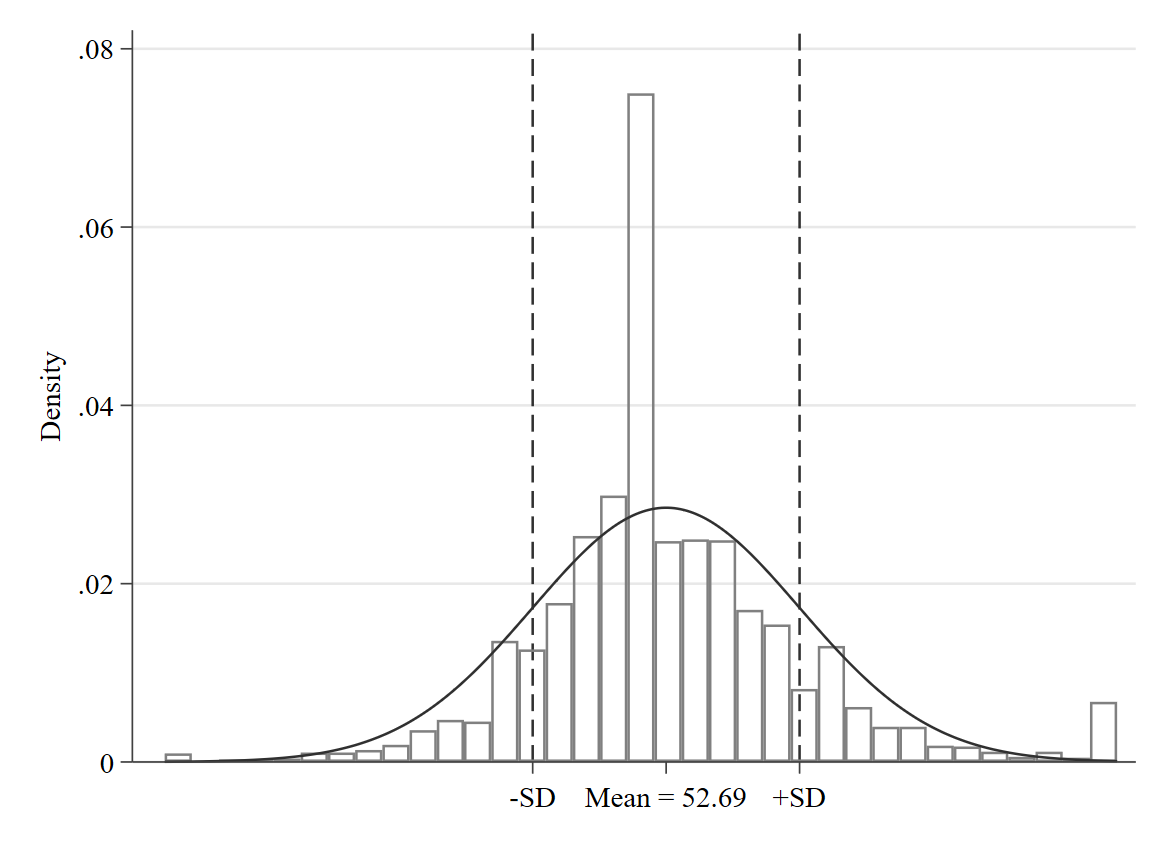
\includegraphics[scale=0.3]{Figures/groupsHist.png}
\end{figure}


\begin{table}[H]
	\centering
	\caption{Groups of incumbent's potential voters according to its level of Affective Polarization}
	\label{tab:groups}
	\begin{tabular}{@{}lcc@{}}
		\toprule
		           & Observations & Percentage \\ \midrule
		Supporters & 18           & 2.21       \\
		Partisans  & 521          & 64.08      \\
		Fans       & 274          & 33.70      \\
		Total      & 813          & 100.00     \\ \bottomrule
	\end{tabular}
\end{table}

In order to explore the data a bit before I turn to the models, I first include two general pictures of the affective polarization index distribution. One distinguishing between government and opposition partisans\footnote{Here everyone who is not a government partisan, is considered a opposition partisan. However, I am considering to include a graph in the appendix desegregating this category with partisan of the opposition and those without a partisan identity.} (Figure \ref*{fig:AP_partisan}) and a second one distinguishing by party identity (Figure \ref*{fig:AP_party_id}). These descriptive data are intended to serve as a general picture of Affective Polarization in Spain provided that this dataset is one of the few available to this day to study such patterns. Although the main goal of the paper is to explore the intensity of economic voting conditional on polarization level and I should focus on incumbent's voters, I think that it is valuable to compare some groups in order to have some insight before I estimate my equations.

We can see that the distribution of the Affective Polarization Index is quite normal for both the incumbent voters and opposition voters. However, it is interesting to see that incumbent voters (Mean = 4.812; SE = 0.03) are significantly more polarized on average than opposition ones (Mean = 3.812; SE = 0.02) (Diff = 1.01; SE = 0.05).

\begin{figure}[H]
	\centering
	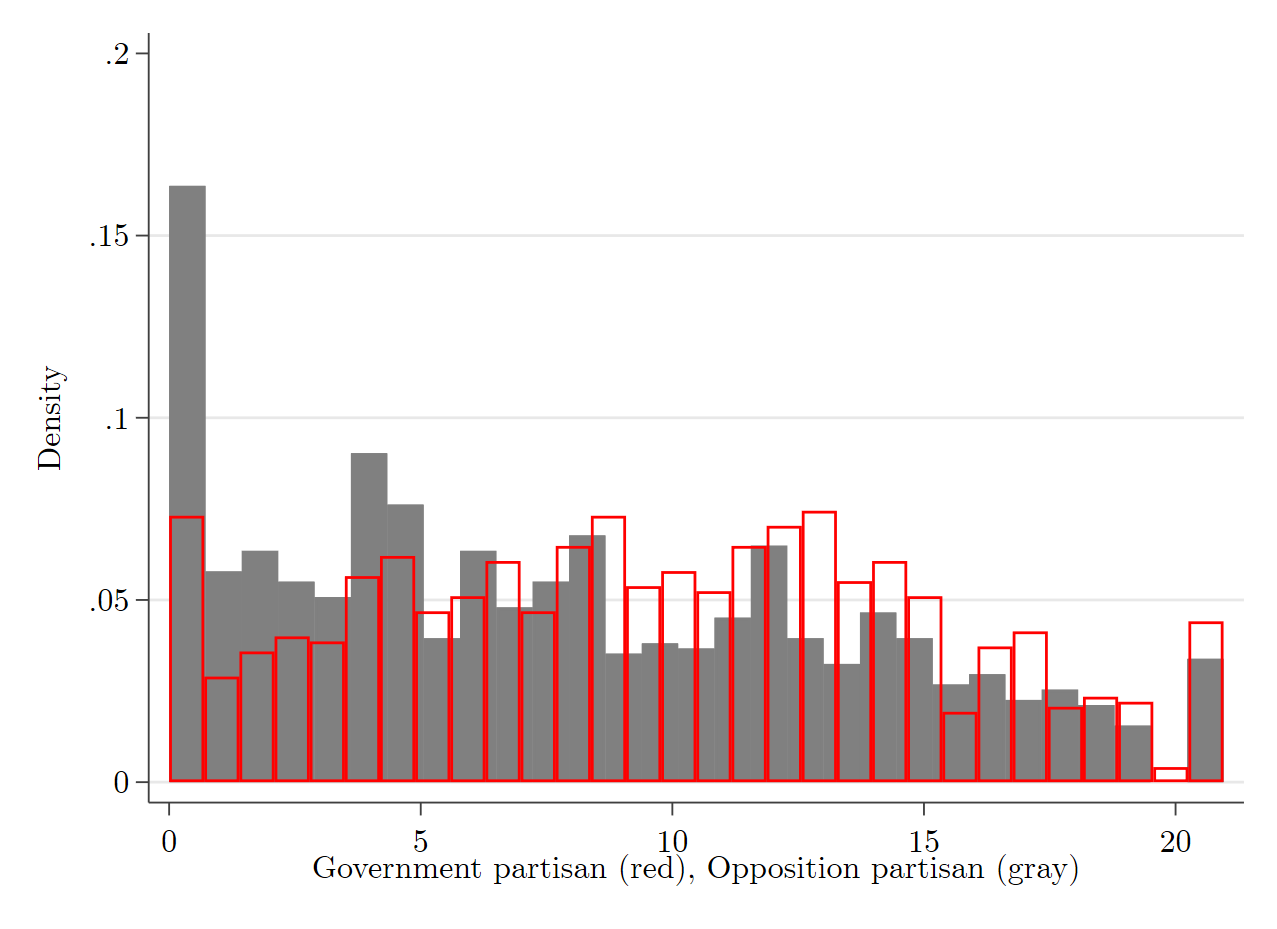
\includegraphics[scale=0.25]{Figures/AP_index_by_partisanship.png}
	\caption{\label{fig:AP_partisan} Affective Polarization Index by partisanship}
\end{figure}

If we take a look now at the distribution of polarization by party (Figure \ref*{fig:AP_party_id}), we also observe some interesting patterns. First, distributions look more similar compared to each other than opposition vs incumbent voters, that is, all parties seem to display a normal distribution of affectively polarized voters. Nevertheless, we can see that mainstream parties (PP and PSOE) are slightly more polarized on average than the rest. However, if we take a look at the distances between these means\footnote{All the descriptive statistics can be found tabulated in the Appendix}, we find that PSOE voters are significantly more polarized than Vox (Diff = 0.704; $p < 0.000$), Unidas Podemos (Diff = 0.312; $p < 0.000$) and Ciudadanos (Diff = 0.654; $p < 0.000$) voters, but PP and Unidas Podemos voters are also significantly more polarized than Vox (Diffs = 0.578 and 0.392 respectively; $p<0.000$) and Ciudadanos (Diffs = 0.528 and 0.342 respectively; $p<0.000$) voters.

These patters might look random at first glance but interestingly enough they could be talking about the dynamics of positive and negative partisanship to a great extent. First, mainstream parties convinced voters (recall that I plot here party identification) usually tend to be against everyone else since they are usually moderate voters. On the one hand, they are against the other side of the spectrum and at the same time, they are against the extreme portion of the same part of the spectrum. Unidas Podemos and Ciudadanos voters should be less polarized since sometimes they are grouped into the so-called ``nueva política (new politics)'' and hence, negative partisanship shouldn't be that large. In the same vein, Vox voters are usually close to PP voters and I think that positive partisanship is driving the distribution if positive partisanship is so important, negative partisanship can be irrelevant if voters are equally far from all the parties.

\begin{figure}[H]
	\centering
	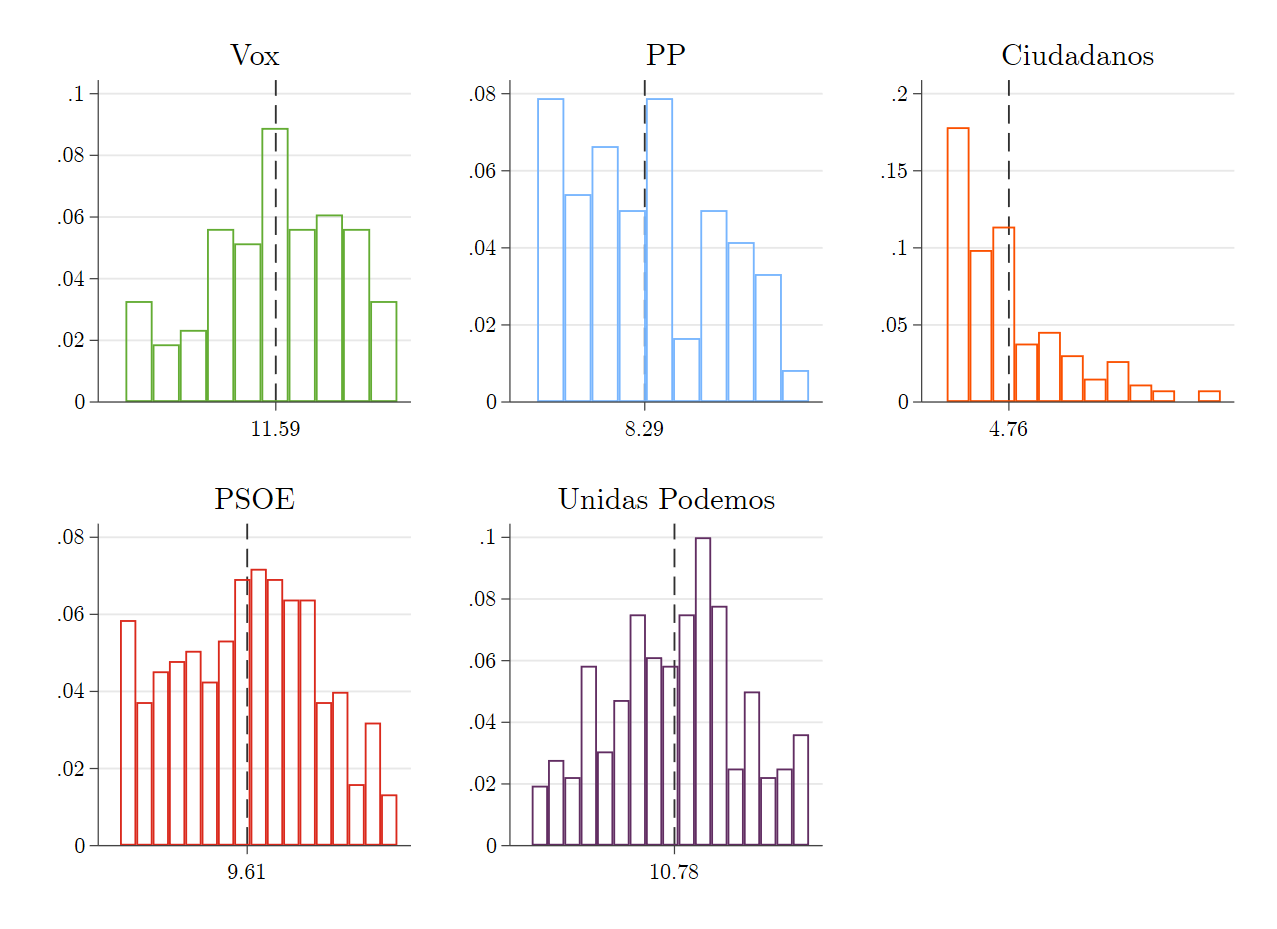
\includegraphics[scale=0.30]{Figures/AP_index_by_party_id.png}
	\caption{\label{fig:AP_party_id} Affective Polarization Index by party identification}
\end{figure}

In Figure \ref*{fig:feelings} we can see the distance in feelings towards voters of each party for those whose level of affective polarization is above and below the average. This is an important measure because reveals the extent to which positive and negative partisanship is present in the Spanish system. The horizontal axis plots the level of warmness that an individual has regarding voters of every one of the four biggest parties. It ranges from 0 being feeling very cold to 100 being feeling very close or warm. In the vertical axis I separate the results for each party to explore the plausible heterogeneity. The parties are ordered according to their position in the ideological scale (left to right is top to bottom) in order to ease the interpretation of the results. The results are somewhat mixed although they can give us some insight to explain later the main empirical findings.

First of all, there is a common pattern among parties and their supporters. Although we could expect that those more polarized than the average have stronger sympathy for their party's voters (i.e. positive partisanship) we rather see that this is only the case for leftwing parties. PSOE and UP voters are significantly warmer towards its copartisans, but also towards the leftwing parties as a whole. Interestingly, none of the remaining parties' voters display a significant increase in positive feelings towards their copartisans the more polarized they are. However, we see some interesting patterns if we now look to the right of the ideological spectrum. PP and Vox voters are significantly warmer towards the other party voters the more polarized they are. That is as if they would define their in-group as composed by the rightwing parties as a whole. Moreover, they also share a special dislike for PSOE (the incumbent most of the time analyzed) voters. Finally, Ciudadnos voters only seem to dislike specially PSOE voters, the remaining distances are not significantly different from zero at the 95\% level.

\begin{figure}[H]
	\centering
	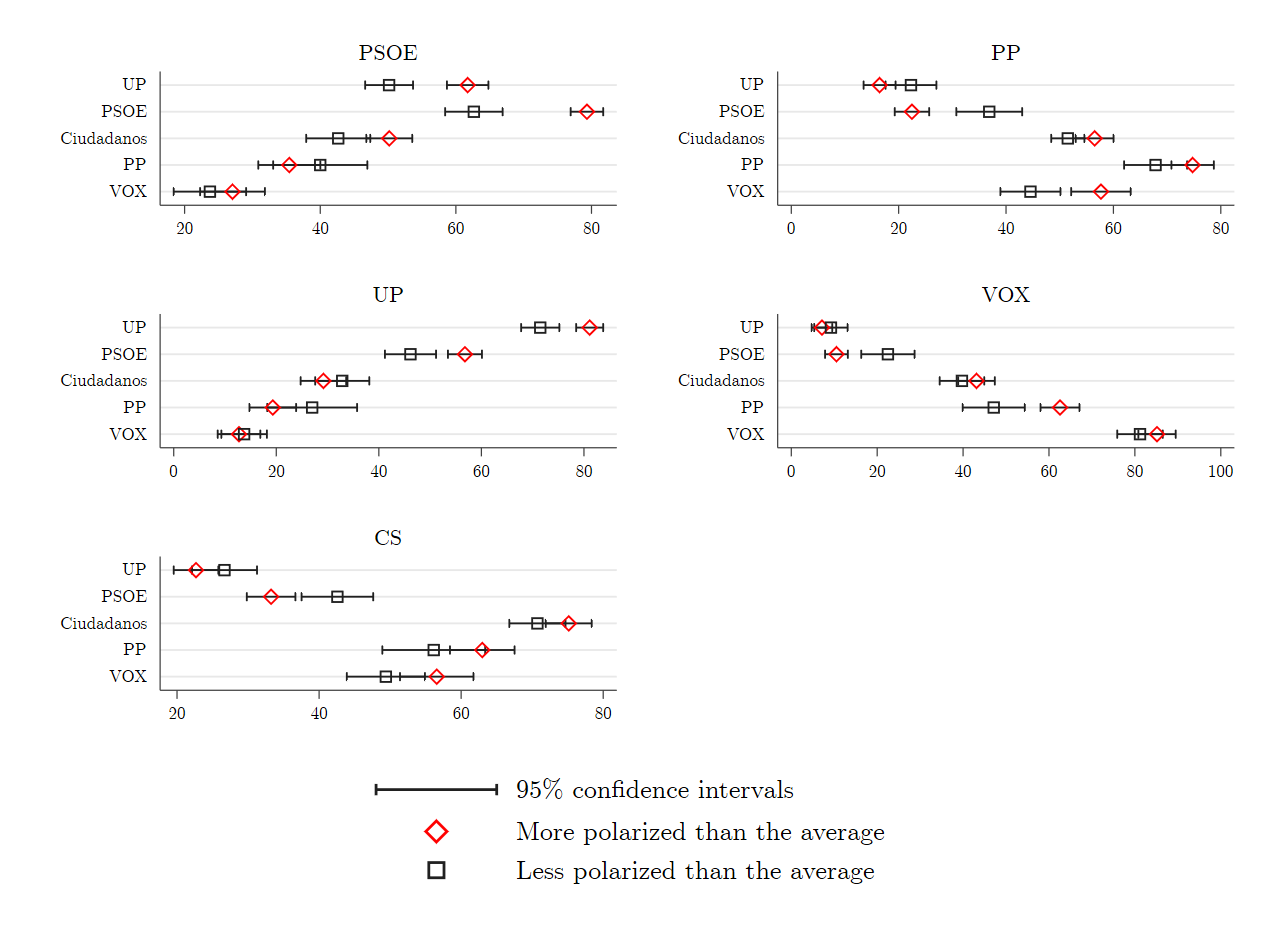
\includegraphics[scale=0.35]{Figures/combinedfeelingsAP.png}
	\caption{\label{fig:feelings} Feelings towards party voters and affective polarization}
\end{figure}

The reason behind plotting parties ordered by ideology in the vertical axis is to better see that except for Ciudadanos who is put at the end of the panel on purpose, we see a mirror image on the pattern. In line with \citep*{Orriols2020}, there is a clear pattern regarding the out-group formation that basically has to do with two ideological blocks. If we look at Figure \ref*{fig:feelings} by rows, we see that left parties' voters display feelings that are a mirror image of those of the rightwing voters. Moreover, the spread of those feelings, in line with \citep*{Wagner2021} is grater as the parties move apart ideologically, that is, feelings towards both the in-group and the  out-group are more extreme for UP and VOX voters than they are for PSOE and PP respectively. Interestingly enough, we also see that PSOE and UP supporters are significantly warmer towards their in-group when they are more polarized whereas PP and VOX supporters tend to be colder towards their out-group the more polarized they are. This suggests that positive partisanship is stronger on the left whereas negative partisanship tend to be stronger on the right.

\subsubsection{Economic assessment}

Now, In order to check if economic voting `is working' as expected, I need a measure of national economy assessment made by respondents. E-DEM dataset includes the arguably most straightforward and common question about economic assessment. Respondents are not asked to give a very precise assessment of the economic situation, they are just asked if they think economy is either better or worse than in the last 12 months.
The variable as it appears in the dataset takes on values 1 (``A lot worse'') to 5 ``A lot better''. I recode this variable to be an index ranging from -2 to 2 so positive values of the index represents positive assessments of the economy and vice-versa.

% Please add the following required packages to your document preamble:
% \usepackage{booktabs}
\begin{table}[H]
	\centering
	\caption{Assessment of the Spanish economy}
	\label{tab:economic assessment}
	\begin{tabular}{@{}lcc@{}}
		\toprule
		                & Observations & Percentage \\ \midrule
		A lot worse     & 654          & 11.68      \\
		A little worse  & 1,271        & 22.70      \\
		No difference   & 2,326        & 41.54      \\
		A little better & 1,314        & 23.47      \\
		A lot better    & 34           & 0.61       \\
		Total           & 5,599        & 100.00     \\ \bottomrule
	\end{tabular}
\end{table}

\subsubsection{Control variables}
My control variables are common sociodemographic controls that might influence the likelihood of voting for the incumbent. They are the region (autonomous community) the individual comes from, sex, age, size of the habitat individual lives, martial status, educational level attained, occupation, income and religious beliefs.

\subsection{Models}

The general model to be estimated is as follows:

\begin{equation}
	\label{model}
	y_i = \beta_1 x_{1i} + \beta_2 x_{2i} + \beta_3 Z_i  + \eta_i  + \epsilon_i
\end{equation}

where $y_i$ is a dummy variable taking on value 1 if the respondent will vote for the incumbent in the following election and 0 otherwise\footnote{For respondents in wave 4, since there is no question asking about a hypothetical future election, a 1 represents people with a score of more than 5 in the question about the probability of ever voting for either PSOE or Unidas Podemos (Podemos+IU)}, $\beta_1$ is the expected effect of economic voting (i.e. the likelihood of voting for the incumbent according to economic assessment) alone, $\beta_2$ is the effect of affective polarization\footnote{In some specifications, this variable is a continuous measure, in others it is a dichotomous one, splitting the sample between those above and those below the average level of affective polarization} on the probability of voting for the incumbent and, the outcome of interest, $\beta_3$ is the interaction between both $x_1$ and $x_2$. Thus, $\beta_3$ capture the effect of economic voting according to the level of affective polarization of the individual. Finally, $\eta_i$ is a vector of sociodemographic control variables, and $\epsilon$ is the error term.


\section{Results}

Now we turn to the main results of the paper. In this section I summarize and discuss the empirical evidence for or against my main hypotheses:

\textit{H1: The more affectively polarized an individual is, the less important is his/her economic assessment to understand his/her likelihood of voting for the incumbent in a future election.}

\textit{H2: Among those who assess the economy as \textbf{worse} than in the past, \textbf{fans} are \textbf{more} willing to vote for the incumbent than partisans and supporters respectively.}

\textit{H3: Among those who assess the economy as \textbf{better} than in the past, \textbf{supporters} are \textbf{less} willing to vote for the incumbent than partisans and fans respectively.}

\begin{table}[H]
	\label{coefplot}
	\centering
	\caption{\label{tab:preferred_model} Effects of affective polarization on economic voting (preferred specification)}
	{
\def\sym#1{\ifmmode^{#1}\else\(^{#1}\)\fi}
\begin{tabular}{l*{3}{c}}
\toprule
                &\multicolumn{3}{c}{Likelihood of voting for the incumbent}\\\cmidrule(lr){2-4}
                & Baseline         &+ Sociodemografic controls         &     est3         \\
\midrule
Economic assessment&   0.0778         &    0.963         &    1.084         \\
                &   (0.84)         &   (1.30)         &   (1.31)         \\
Partisans       &                  &    1.666\sym{*}  &    1.654\sym{*}  \\
                &                  &   (2.47)         &   (2.31)         \\
Fans            &                  &    2.527\sym{**} &    2.572\sym{**} \\
                &                  &   (2.95)         &   (2.90)         \\
Partisans $\times$ Economic assessment&                  &   -0.333         &   -0.469         \\
                &                  &  (-0.42)         &  (-0.54)         \\
Fans $\times$ Economic assessment&                  &   -1.445         &   -1.582         \\
                &                  &  (-1.51)         &  (-1.56)         \\
Region          &                  &                  &   0.0175         \\
                &                  &                  &   (0.45)         \\
Sex             &                  &                  &   -0.352         \\
                &                  &                  &  (-0.90)         \\
Age             &                  &                  &  -0.0310         \\
                &                  &                  &  (-1.80)         \\
Habitat (Nr. of inhabitants)&                  &                  &    0.473\sym{*}  \\
                &                  &                  &   (1.96)         \\
Marital Status  &                  &                  &   0.0367         \\
                &                  &                  &   (0.36)         \\
Education level &                  &                  &   -0.181         \\
                &                  &                  &  (-1.25)         \\
Occupation      &                  &                  &   0.0331         \\
                &                  &                  &   (0.38)         \\
Income          &                  &                  &   0.0244         \\
                &                  &                  &   (0.33)         \\
Belongs to a church&                  &                  &   -0.475         \\
                &                  &                  &  (-1.26)         \\
Constant        &    1.127\sym{***}&    1.406\sym{*}  &    3.206\sym{*}  \\
                &  (14.44)         &   (2.20)         &   (2.06)         \\
\midrule
Pseudo \(R^{2}\)&    0.001         &    0.064         &    0.109         \\
Observations    &     1037         &      812         &      812         \\
\bottomrule
\multicolumn{4}{l}{\footnotesize \textit{t} statistics in parentheses}\\
\multicolumn{4}{l}{\footnotesize \sym{*} \(p<0.05\), \sym{**} \(p<0.01\), \sym{***} \(p<0.001\)}\\
\end{tabular}
}


\end{table}

\begin{figure}[H]
	\centering
	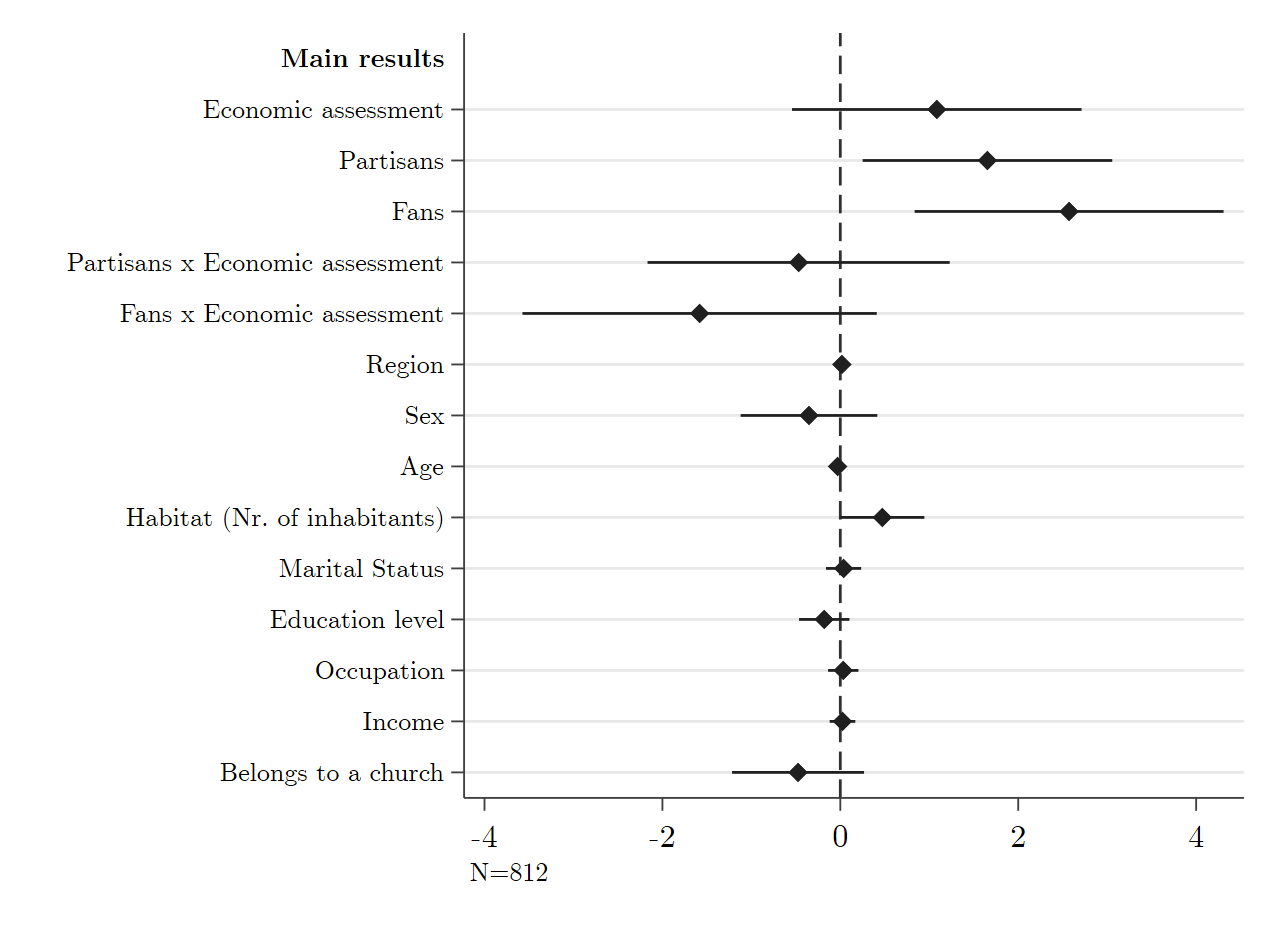
\includegraphics[scale=0.35]{Figures/new.png}
	\caption{\label{fig:preferred_model} Economic voting and affective polarization}
\end{figure}

\begin{figure}[H]
	\centering
	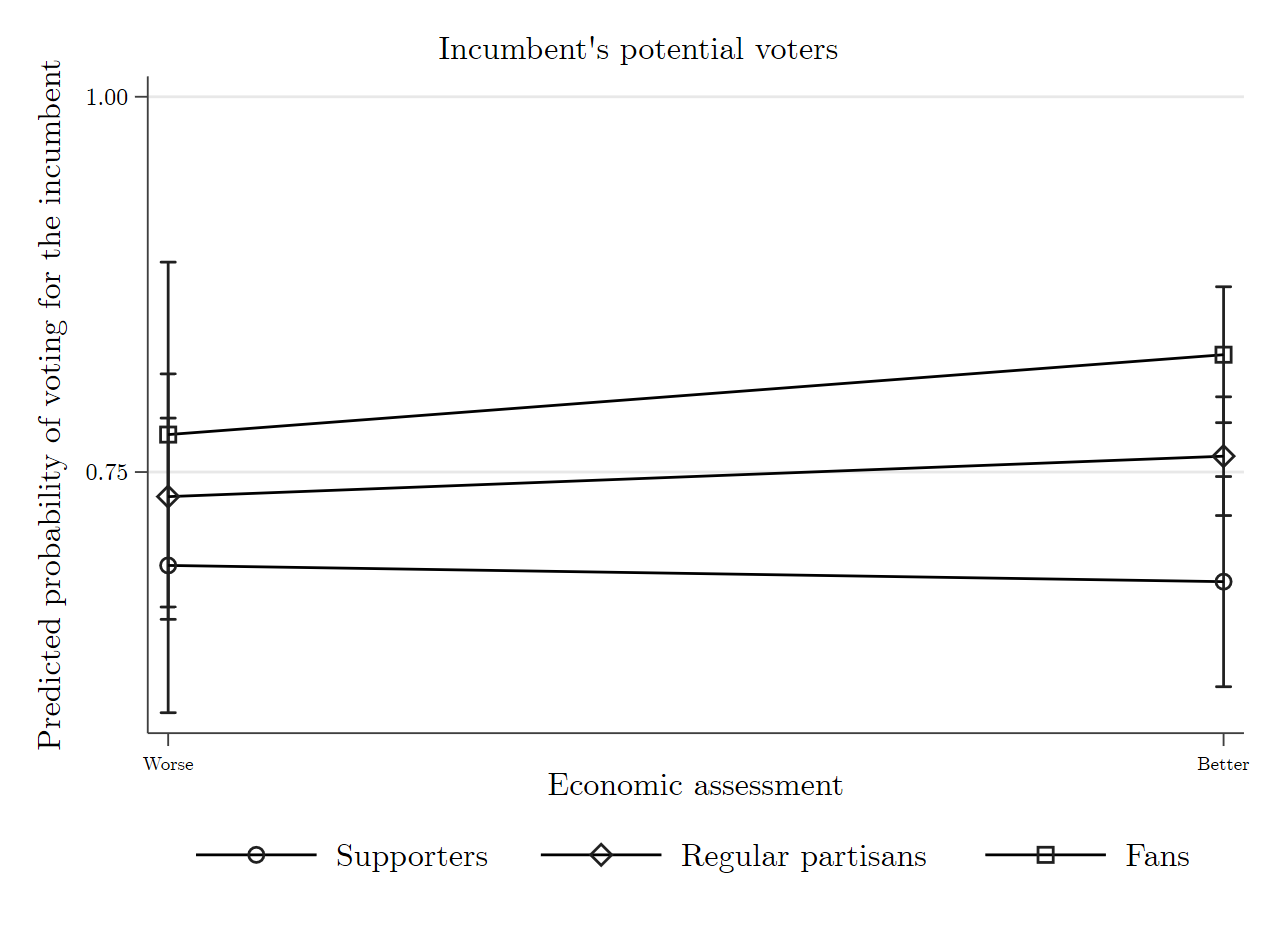
\includegraphics[scale=0.35]{Figures/margins.png}
	\caption{\label{fig:margins} Economic voting and affective polarization}
\end{figure}

% As we can see in Table \ref*{tab:preferred_model} I present the results of estimating equation \ref*{model}\footnote{To have a notion of the magnitude of the effects, in future iterations of the paper I will present odds ratios in the appendix.} first without controls and then adding common sociodemographic controls. In the two models, the effect of economic voting is positive as expected, meaning that those that evaluate the economy as better than in the last twelve months, are more likely to vote for the incumbent. Furthermore, the affective polarization index measured (following \citep*{Wagner2021}) as the weighted average party affect difference compared to each respondent's weighted average party affect has a negative and significant effect on the likelihood of voting for the incumbent. This measure though is not useful alone since its interpretation is not easy, hence, I provide marginal effects in section \ref*{section:margins} to explore the different possible patterns.

% The main quantity of interest, namely, the interaction between these two terms, is significant at the 99.9\% level (even after controlling for a set of sociodemographic control variables) and its effect is negative which constitute empirical support for the general hypothesis since it would mean that as people is more polarized, they are less able to use economic voting in the proper (or rational) way. In other words, this flip in the signs of $\beta_1$ and $\beta_2$ would suggest that, according to my theoretical expectations, those more polarized are less able to vote critically. To better see the results I also provide an alternative way of presenting the results in Figure \ref*{fig:preferred_model}

% Finally, in order to see different possible specifications I provide now models with a continuous and a dichotomous version of the Affective Polarization index. Moreover, I also provide models desegregating by party identification instead of splitting between incumbent and opposition supporters. I have to say in advance that only the model with the dichotomous measure and opposition vs incumbent supporters yields statistically significant results.

% \begin{table}[H]
% 	\label{coefplot}
% 	\centering
% 	\caption{\label{tab:preferred_model} Effects of affective polarization on economic voting (preferred specification)}
% 	{
\def\sym#1{\ifmmode^{#1}\else\(^{#1}\)\fi}
\begin{tabular}{l*{5}{c}}
\toprule
                &\multicolumn{5}{c}{Likelihood of voting for the incumbent}                                    \\\cmidrule(lr){2-6}
                & Baseline         &+ Sociodemografic controls         &     est3         &     est4         &     est5         \\
\midrule
Economic assessment&   0.0778         &    0.963         &    1.084         &    0.459\sym{***}&    0.431\sym{***}\\
                &   (0.84)         &   (1.30)         &   (1.31)         &   (6.55)         &   (5.92)         \\
Supporters      &                  &        0         &        0         &                  &                  \\
                &                  &      (.)         &      (.)         &                  &                  \\
Partisans       &                  &    1.666\sym{*}  &    1.654\sym{*}  &                  &                  \\
                &                  &   (2.47)         &   (2.31)         &                  &                  \\
Fans            &                  &    2.527\sym{**} &    2.572\sym{**} &                  &                  \\
                &                  &   (2.95)         &   (2.90)         &                  &                  \\
Supporters $\times$ Economic assessment&                  &        0         &        0         &                  &                  \\
                &                  &      (.)         &      (.)         &                  &                  \\
Partisans $\times$ Economic assessment&                  &   -0.333         &   -0.469         &                  &                  \\
                &                  &  (-0.42)         &  (-0.54)         &                  &                  \\
Fans $\times$ Economic assessment&                  &   -1.445         &   -1.582         &                  &                  \\
                &                  &  (-1.51)         &  (-1.56)         &                  &                  \\
Sociodemografic controls&                  &                  &                  &                  &                  \\
Region          &                  &                  &   0.0175         &                  & -0.00793         \\
                &                  &                  &   (0.45)         &                  &  (-0.67)         \\
Sex             &                  &                  &   -0.352         &                  &   0.0925         \\
                &                  &                  &  (-0.90)         &                  &   (0.82)         \\
Age             &                  &                  &  -0.0310         &                  & -0.00293         \\
                &                  &                  &  (-1.80)         &                  &  (-0.55)         \\
Habitat (Nr. of inhabitants)&                  &                  &    0.473\sym{*}  &                  &   0.0466         \\
                &                  &                  &   (1.96)         &                  &   (0.73)         \\
Marital Status  &                  &                  &   0.0367         &                  &   0.0332         \\
                &                  &                  &   (0.36)         &                  &   (1.20)         \\
Education level &                  &                  &   -0.181         &                  &   0.0386         \\
                &                  &                  &  (-1.25)         &                  &   (0.92)         \\
Occupation      &                  &                  &   0.0331         &                  & -0.00619         \\
                &                  &                  &   (0.38)         &                  &  (-0.22)         \\
Income          &                  &                  &   0.0244         &                  &  -0.0702\sym{***}\\
                &                  &                  &   (0.33)         &                  &  (-3.31)         \\
Belongs to a church&                  &                  &   -0.475         &                  &   -0.542\sym{***}\\
                &                  &                  &  (-1.26)         &                  &  (-4.48)         \\
AP index (dichotomous)&                  &                  &                  &   -3.455\sym{***}&   -3.470\sym{***}\\
                &                  &                  &                  & (-19.22)         & (-19.28)         \\
Economic assessment $\times$ AP index (dichotomous)&                  &                  &                  &   -0.792\sym{***}&   -0.793\sym{***}\\
                &                  &                  &                  &  (-4.91)         &  (-4.87)         \\
Opposition supporter&                  &                  &                  &   -2.228\sym{***}&   -2.220\sym{***}\\
                &                  &                  &                  & (-11.91)         & (-11.67)         \\
Constant        &    1.127\sym{***}&    1.406\sym{*}  &    3.206\sym{*}  &    1.326\sym{***}&    1.539\sym{***}\\
                &  (14.44)         &   (2.20)         &   (2.06)         &   (7.21)         &   (3.40)         \\
\midrule
Pseudo \(R^{2}\)&    0.001         &    0.064         &    0.109         &    0.280         &    0.295         \\
Observations    &     1037         &      812         &      812         &     3737         &     3737         \\
\bottomrule
\multicolumn{6}{l}{\footnotesize \textit{t} statistics in parentheses}\\
\multicolumn{6}{l}{\footnotesize NOTE: The AP dichotomous variable splits the sample between those avobe and below the average AP level.}\\
\multicolumn{6}{l}{\footnotesize \sym{*} \(p<0.05\), \sym{**} \(p<0.01\), \sym{***} \(p<0.001\)}\\
\end{tabular}
}


% \end{table}

% \begin{figure}[H]
% 	\centering
% 	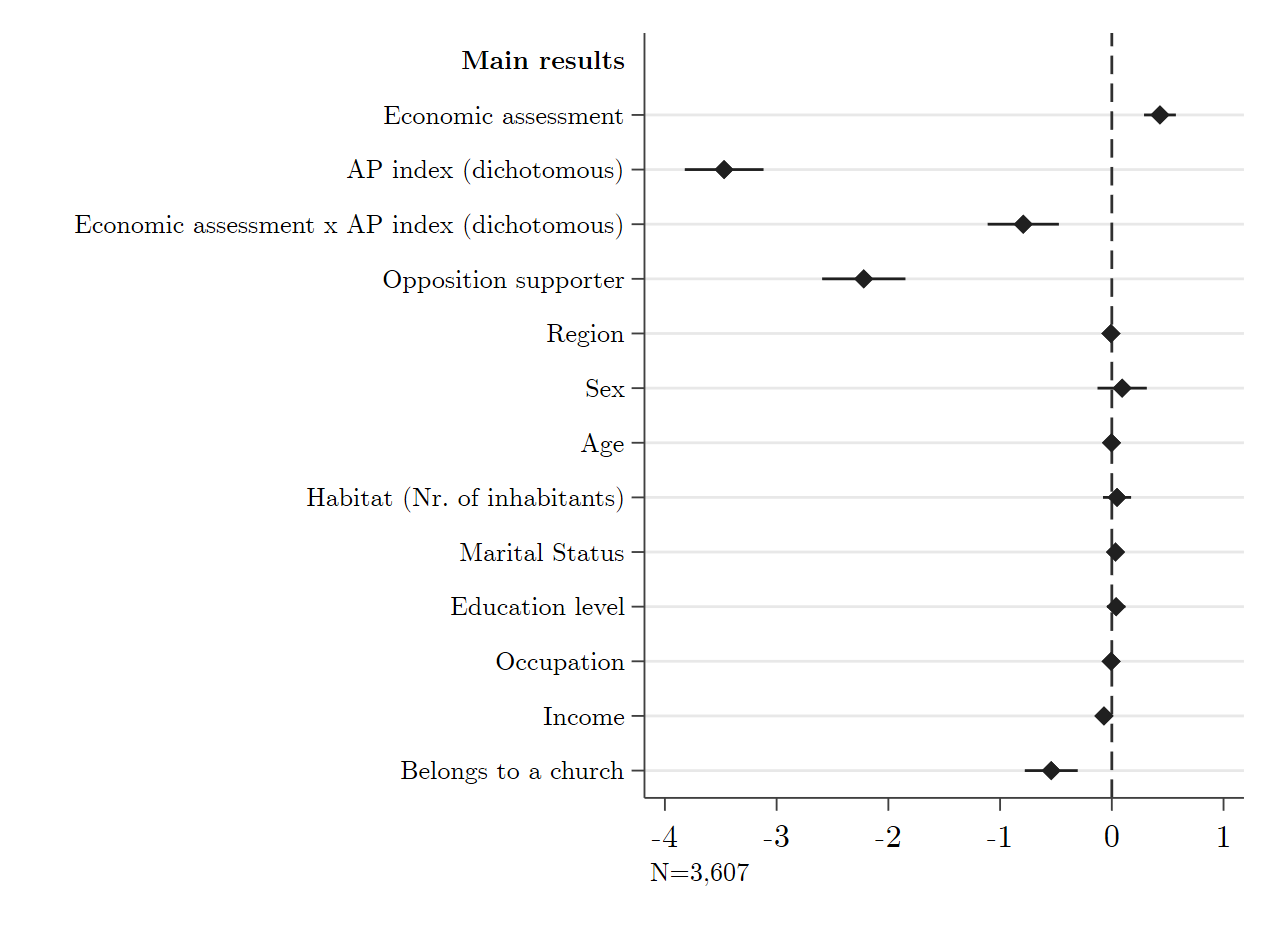
\includegraphics[scale=0.35]{Figures/preferred_model.png}
% 	\caption{\label{fig:preferred_model} Economic voting and affective polarization (Preferred Specification)}
% \end{figure}

% \begin{table}[H]
% 	\centering
% 	\caption{\label{tab:continue_opposition} Effects of affective polarization on economic voting (AP index continuous and opposition vs incumbent)}
% 	{
\def\sym#1{\ifmmode^{#1}\else\(^{#1}\)\fi}
\begin{tabular}{l*{2}{c}}
\toprule
                &\multicolumn{2}{c}{Likelihood of voting for the incumbent}\\\cmidrule(lr){2-3}
                & Baseline         &+ Sociodemografic controls         \\
\midrule
Economic assessment&    0.435\sym{*}  &    0.434\sym{*}  \\
                &   (2.34)         &   (2.30)         \\
AP index        &    0.205\sym{***}&    0.247\sym{***}\\
                &   (5.18)         &   (6.07)         \\
Economic assessment $\times$ AP index&   0.0180         &-0.000288         \\
                &   (0.42)         &  (-0.01)         \\
Opposition supporter&   -3.785\sym{***}&   -3.786\sym{***}\\
                & (-20.31)         & (-20.17)         \\
\midrule
Pseudo \(R^{2}\)&    0.319         &    0.333         \\
Observations    &     3459         &     3459         \\
\bottomrule
\multicolumn{3}{l}{\footnotesize \textit{t} statistics in parentheses}\\
\multicolumn{3}{l}{\footnotesize \sym{*} \(p<0.05\), \sym{**} \(p<0.01\), \sym{***} \(p<0.001\)}\\
\end{tabular}
}


% \end{table}

% \begin{table}[H]
% 	\centering
% 	\caption{\label{tab:dummy_parties} Effects of affective polarization on economic voting (AP index dichotomous and party ID)}
% 	{
\def\sym#1{\ifmmode^{#1}\else\(^{#1}\)\fi}
\begin{tabular}{l*{2}{c}}
\toprule
                &\multicolumn{2}{c}{Likelihood of voting for the incumbent}\\\cmidrule(lr){2-3}
                & Baseline         &+ Sociodemografic controls         \\
\midrule
Economic assessment&    0.310         &    0.253         \\
                &   (1.63)         &   (1.29)         \\
AP index (dichotomous)&   -5.139\sym{***}&   -5.238\sym{***}\\
                & (-11.44)         & (-11.21)         \\
Economic assessment $\times$ AP index (dichotomous)&   0.0503         &   0.0970         \\
                &   (0.11)         &   (0.20)         \\
Ref. category: PSOE (incumbent)&                  &                  \\
VOX             &   -5.561\sym{***}&   -5.441\sym{***}\\
                &  (-5.24)         &  (-5.06)         \\
PP              &   -4.153\sym{***}&   -4.059\sym{***}\\
                &  (-5.18)         &  (-4.95)         \\
Ciudadanos      &   -3.457\sym{***}&   -3.534\sym{***}\\
                &  (-7.88)         &  (-7.77)         \\
UP              &   -1.199\sym{***}&   -1.521\sym{***}\\
                &  (-3.39)         &  (-3.84)         \\
\midrule
Pseudo \(R^{2}\)&    0.555         &    0.565         \\
Observations    &     1145         &     1145         \\
\bottomrule
\multicolumn{3}{l}{\footnotesize \textit{t} statistics in parentheses}\\
\multicolumn{3}{l}{\footnotesize NOTE: The AP dichotomous variable splits the sample between those avobe and below the average AP level.}\\
\multicolumn{3}{l}{\footnotesize \sym{*} \(p<0.05\), \sym{**} \(p<0.01\), \sym{***} \(p<0.001\)}\\
\end{tabular}
}


% \end{table}

% \begin{table}[H]
% 	\centering
% 	\caption{\label{tab:continuous_parties} Effects of affective polarization on economic voting (AP index continuous and party ID)}
% 	{
\def\sym#1{\ifmmode^{#1}\else\(^{#1}\)\fi}
\begin{tabular}{l*{2}{c}}
\toprule
                &\multicolumn{2}{c}{Likelihood of voting for the incumbent}\\\cmidrule(lr){2-3}
                & Baseline         &+ Sociodemografic controls         \\
\midrule
Economic assessment&    0.554         &    0.560         \\
                &   (1.27)         &   (1.27)         \\
AP index        &    0.151         &    0.184\sym{*}  \\
                &   (1.87)         &   (2.23)         \\
Economic assessment $\times$ AP index&  -0.0685         &  -0.0802         \\
                &  (-0.75)         &  (-0.87)         \\
Ref. category: PSOE (incumbent)&                  &                  \\
VOX             &   -5.232\sym{***}&   -5.157\sym{***}\\
                & (-13.35)         & (-12.97)         \\
PP              &   -5.316\sym{***}&   -5.231\sym{***}\\
                & (-14.48)         & (-14.03)         \\
Ciudadanos      &   -4.433\sym{***}&   -4.438\sym{***}\\
                & (-16.60)         & (-16.43)         \\
UP              &   -2.374\sym{***}&   -2.533\sym{***}\\
                & (-11.15)         & (-11.41)         \\
\midrule
Pseudo \(R^{2}\)&    0.446         &    0.450         \\
Observations    &     1682         &     1682         \\
\bottomrule
\multicolumn{3}{l}{\footnotesize \textit{t} statistics in parentheses}\\
\multicolumn{3}{l}{\footnotesize \sym{*} \(p<0.05\), \sym{**} \(p<0.01\), \sym{***} \(p<0.001\)}\\
\end{tabular}
}


% \end{table}


% \newpage

% \subsection*{Marginal Effects}
% \label{section:margins}
% In this section, I provide marginal effects at different levels of economic assessment for each of the specifications above.

% \begin{figure}[H]
% 	\centering
% 	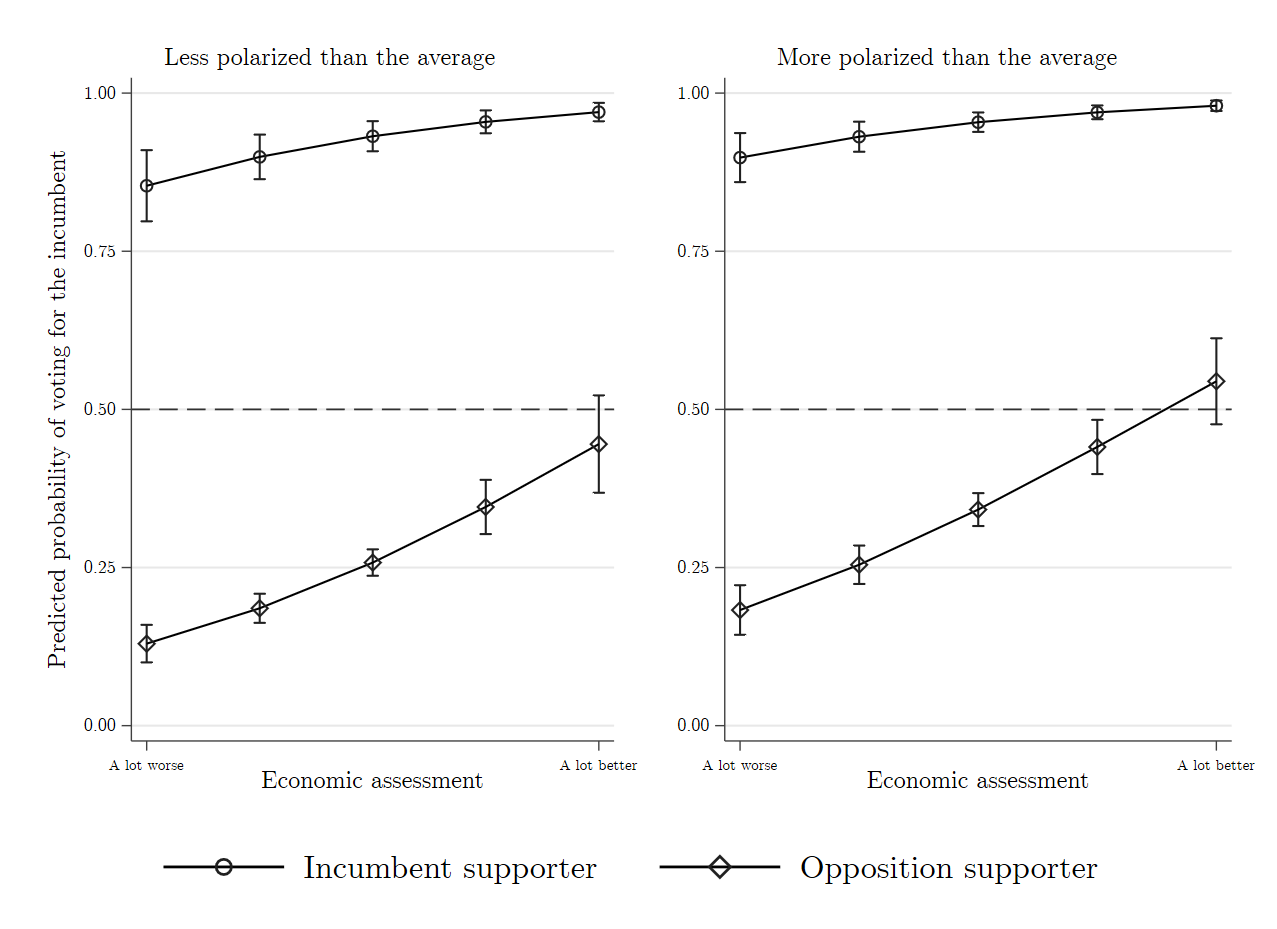
\includegraphics[scale=0.30]{Figures/continue_oppo_incumb.png}
% 	\caption{\label{fig:continue_oppo_incumb} (AP index continuous and opposition vs incumbent)}
% \end{figure}

% \begin{figure}[H]
% 	\centering
% 	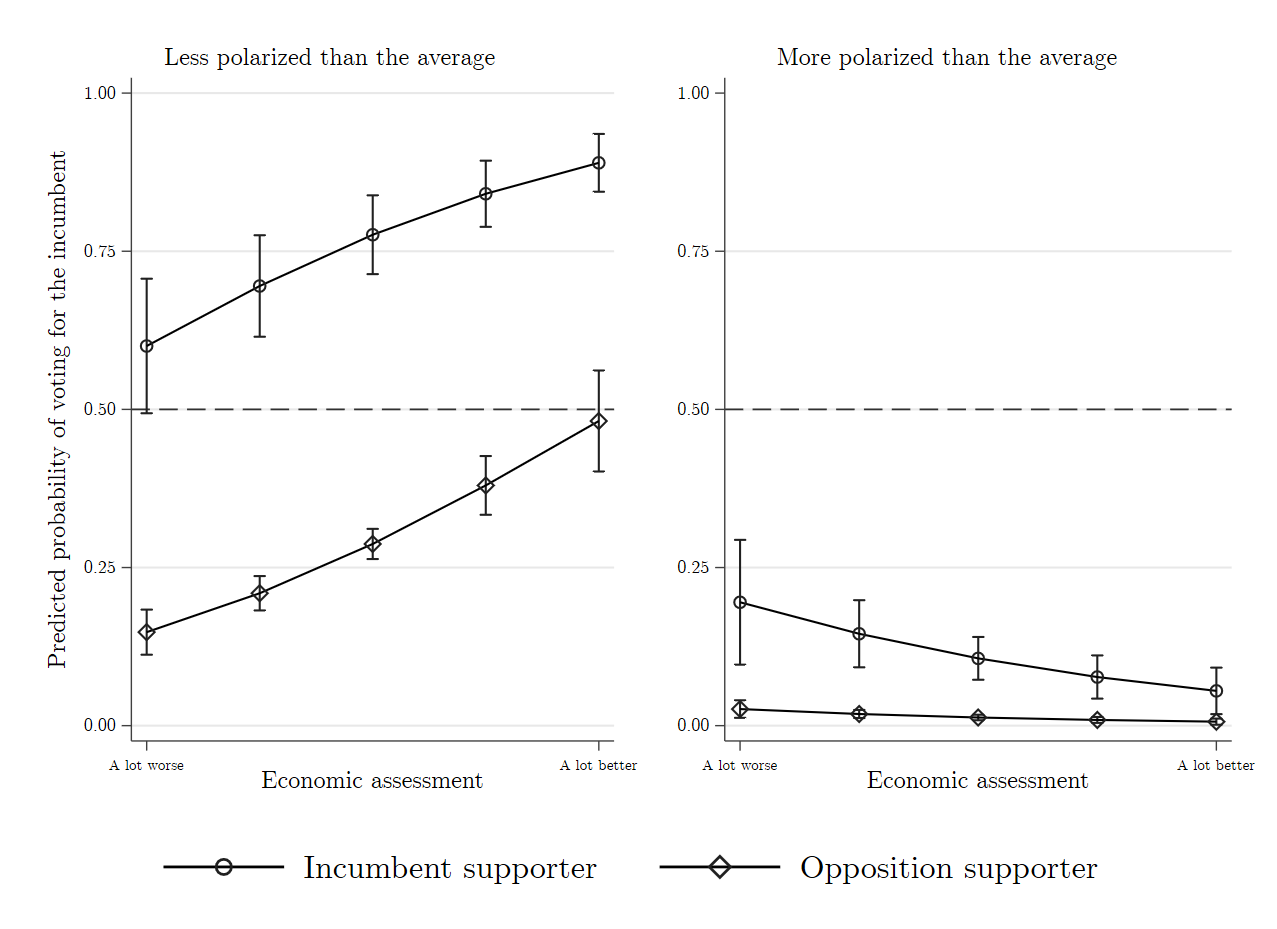
\includegraphics[scale=0.30]{Figures/dummy_oppo_incumb1.png}
% 	\caption{\label{fig:dummy_oppo_incumb1} (AP index dichotomous and opposition vs incumbent)}
% \end{figure}

% \begin{figure}[H]
% 	\centering
% 	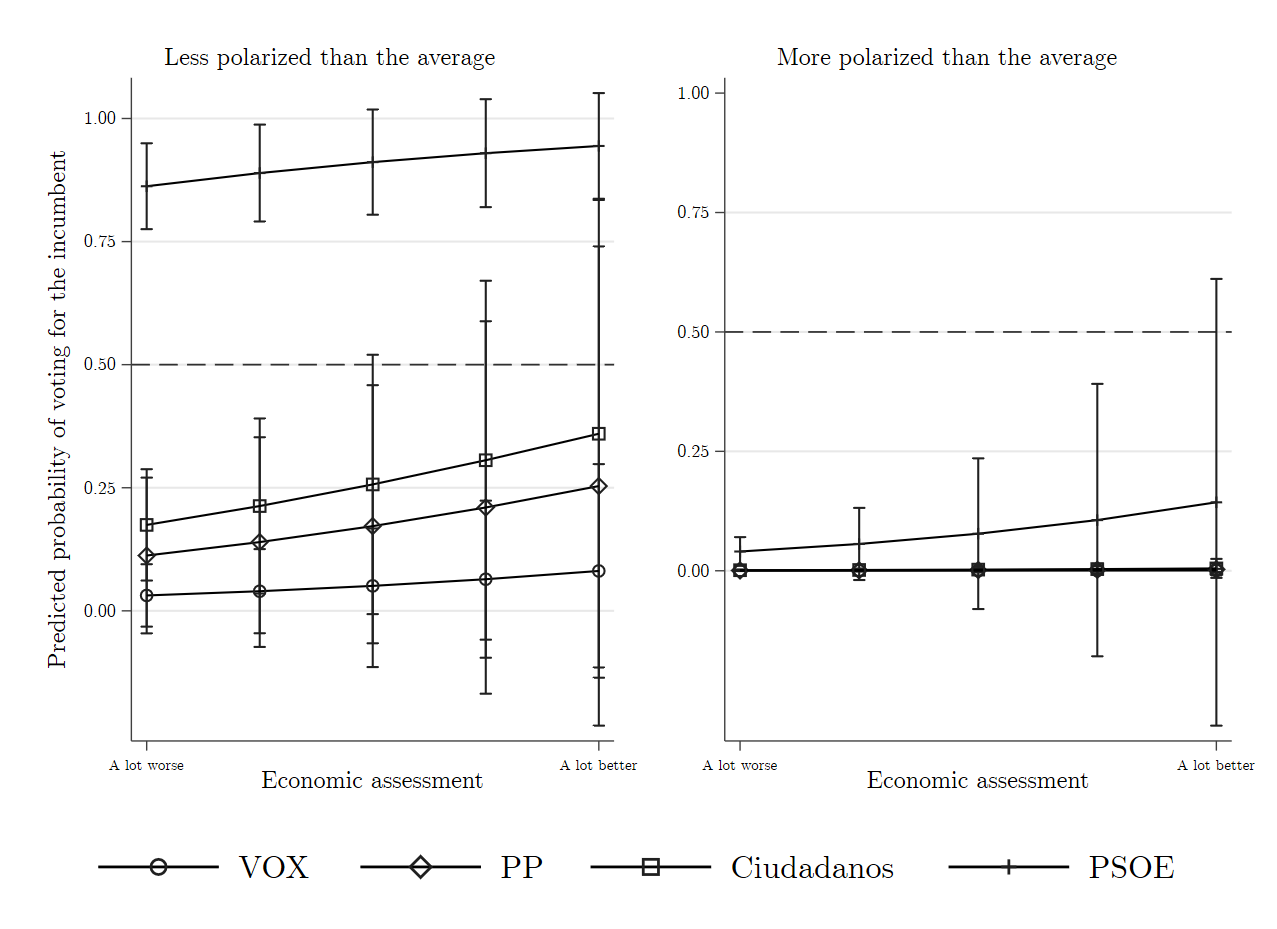
\includegraphics[scale=0.30]{Figures/dummy_parties.png}
% 	\caption{\label{fig:dummy_parties} (AP index dichotomous and party ID)}
% \end{figure}

% \begin{figure}[H]
% 	\centering
% 	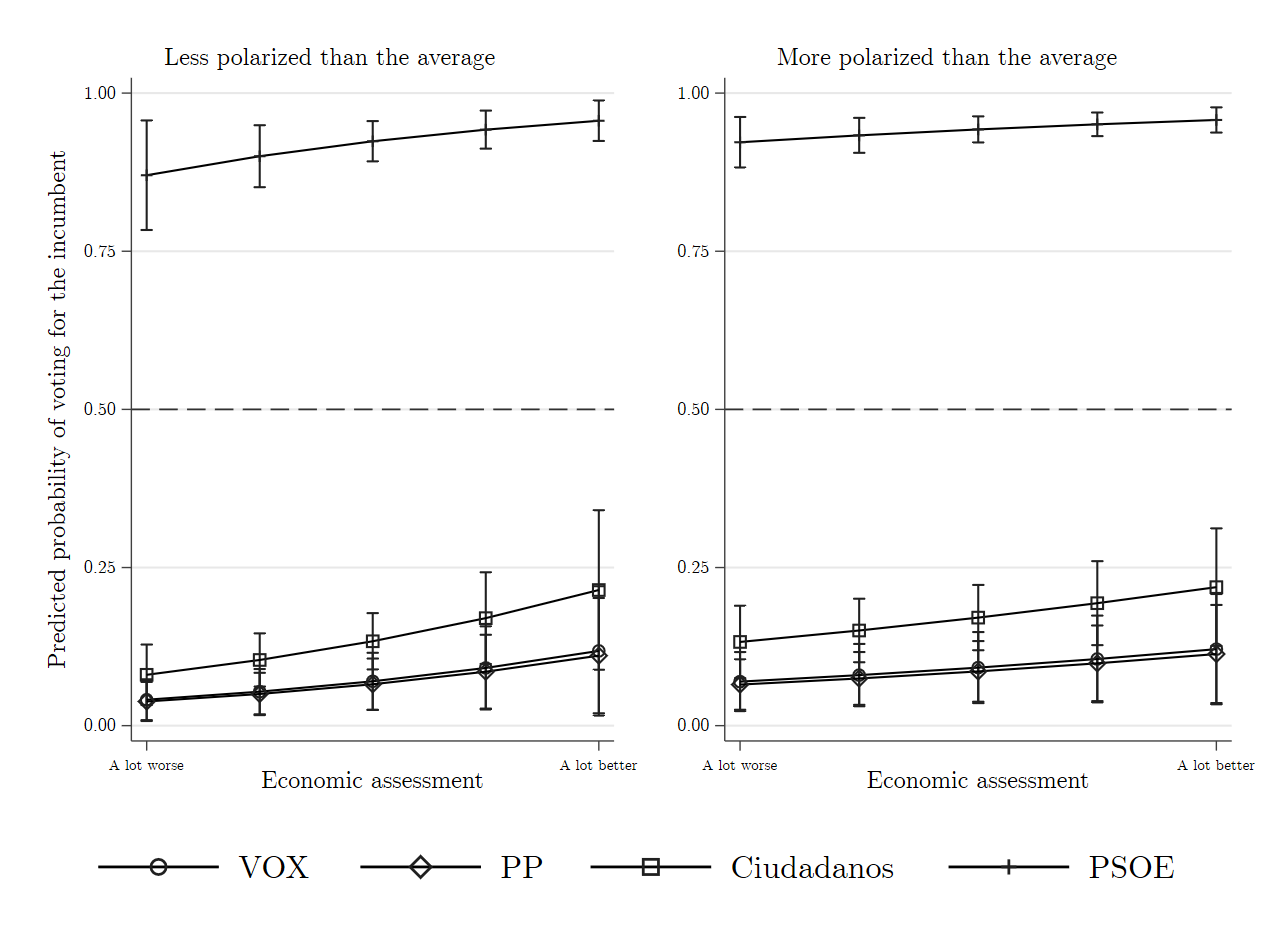
\includegraphics[scale=0.30]{Figures/continue_parties.png}
% 	\caption{\label{fig:continue_parties} (AP index continuous and party ID)}
% \end{figure}


% \section{Broader discussion and possible implications}

% All in all, I think that this paper can contribute to our knowledge about affective polarization as such, and more specifically I can push the  frontier of knowledge forward by analyzing its consequences. This piece of work can have even broader implications since it speaks to the general question of accountability itself. I tend to agree with Robert Fishman that economic voting is not always good. Or, in other words, the fact that polarized people would be less prone to vote ``rationally" according to the economic voting logic is not necessarily something good for our democracies. Nevertheless, looking at the amount of literature proving empirically the importance of economy as a tool for the voter to punish or reward politicians in the government, I still think that economic voting is somewhat related to accountability. Accountability is by no means the only desirable feature of a democratic system, but \textit{ceteris paribus}, it is better to have accountability than not to have it. Moreover, the lack of accountability I predict in this study is related to people's lack of elasticity when it comes to critically analyze the economic situation. If people is not able to punish or reward incumbents due to biases and polarization, in general terms, I would say it is a bad outcome for our democracies.

% I believe that analyzing the consequences of affective polarization and its effects on political attitudes can open an inspiring intellectual debate about the perils of the phenomenon and the available tools we have to avoid the erosion of our democracies.

\newpage
\bibliographystyle{apalike}
\bibliography{RIP.bib}


\newpage

\section*{Appendix}

\begin{table}[H]
	\centering
	\caption{Comparisons of Affective Polarization Index by party identification}
	\label{tab:anova-parties}
	\begin{tabular}{@{}ccccc@{}}
		\toprule
		\multirow{2}{*}{}           & \multirow{2}{*}{VOX} & \multirow{2}{*}{PP} & \multirow{2}{*}{Ciudadanos} & \multirow{2}{*}{PSOE} \\
		                            &                      &                     &                             &                       \\ \midrule
		\multirow{2}{*}{PP}         & 0.578                &                     &                             &                       \\
		                            & 0.000                &                     &                             &                       \\
		\multirow{2}{*}{Ciudadanos} & 0.050                & -0.528              &                             &                       \\
		                            & 0.987                & 0.000               &                             &                       \\
		\multirow{2}{*}{PSOE}       & 0.704                & 0.127               & 0.654                       &                       \\
		                            & 0.000                & 0.586               & 0.000                       &                       \\
		\multirow{2}{*}{UP}         & 0.392                & -0.186              & 0.342                       & -0.312                \\
		                            & 0.000                & 0.188               & 0.000                       & 0.000                 \\ \bottomrule
	\end{tabular}
\end{table}

\end{document}